\documentclass[prd,aps,letterpaper,floatfix,superscriptaddress,preprintnumbers,twocolumn,10pt,nofootinbib]{revtex4-1}


\usepackage{dcolumn}% Align table columns on decimal point
\usepackage{bm}% bold math
\usepackage[dvips]{graphicx}
\usepackage{epsfig}
\usepackage{amsmath, amsfonts, amssymb, slashed}
%\nofile
\usepackage{slashed}
\usepackage{xcolor}
\usepackage{bm}        
\usepackage{graphicx,psfrag,subfigure}
\usepackage{booktabs}
\usepackage[colorlinks]{hyperref}
\usepackage{rotating}
\usepackage{units}
\usepackage{float}

\usepackage{ulem}
\hypersetup{
    colorlinks=true,
    linkcolor=blue,
    filecolor=magenta,      
    urlcolor=cyan,
}
\urlstyle{same}
\def\lsim{\mathrel{\raise.3ex\hbox{$<$\kern-.75em\lower1ex\hbox{$\sim$}}}}
\def\gsim{\mathrel{\raise.3ex\hbox{$>$\kern-.75em\lower1ex\hbox{$\sim$}}}}

\definecolor{red}{rgb}{1.0, 0, 0}
%\newcommand{\draftnote}[1]{{\bf\color{red} \MakeUppercase{#1}}}
%\newcommand{\charan}[1]{{\bf\color{cyan}#1}}
%\newcommand{\veronica}[1]{{\bf\color{green}#1}}

\newcommand{\VS}[2]{{\color{blue}\sout{#1}\textit{#2}}}
\newcommand{\MS}[2]{{\color{red}\sout{#1}\textit{#2}}}
\newcommand{\CK}[2]{{\color{magenta}\sout{#1}\textit{#2}}}


\newcommand{\beqa}{\begin{eqnarray}}
\newcommand{\eeqa}{\end{eqnarray}}

\newcommand{\be}{\begin{equation}}
\newcommand{\ee}{\end{equation}}
\newcommand{\cl}{\%\,\,  \text{C.L.}}

\begin{document}
%\title{On finding collider-stable particles using Machine Learning}
\title{WIMPs or else? Using Machine Learning to disentangle LHC signatures}
%\author{Charanjit K. Khosa, Veronica Sanz and Michael Soughton} 
\author{Charanjit K. Khosa} 
\affiliation{Department of Physics and Astronomy, University of Sussex, 
Brighton BN1 9QH, UK}

\author{Veronica Sanz} 
\affiliation{Department of Physics and Astronomy, University of Sussex, 
Brighton BN1 9QH, UK}
\affiliation{Alan Turing Institute, British Library, 96 Euston Road, London NW1 2DB, UK}
\affiliation{Instituto de F\'isica Corpuscular (IFIC), Universidad de Valencia-CSIC, E-46980, Valencia, Spain}
\author{Michael Soughton} \affiliation{Department of Physics and Astronomy, University of Sussex, 
Brighton BN1 9QH, UK}


\email{charanjit.kaur@sussex.ac.uk}
\email{V.Sanz@sussex.ac.uk}
\email{M.Soughton@sussex.ac.uk}

\date{\today}
\begin{abstract}
We study the prospects of detecting and characterising Dark Matter at colliders using Machine Learning (ML) techniques. We focus on the  monojet and missing transverse energy (MET) channel and propose a set of benchmark models for the study: a typical WIMP Dark Matter candidate in the form of a SUSY neutralino, a pseudo-Goldstone impostor in the shape of an Axion-Like Particle, and a light Dark Matter impostor whose interactions are mediated by a heavy particle. All these benchmarks are tensioned against the main SM background ($Z$+jets) and against each other. Our analysis uses both the leading-order kinematic features as well as the information in additional hard jets. We use different representations of the data, from a simple event data sample with values of kinematic variables fed into a Logistic Regression algorithm or a Neural Network, to a transformation of the data into images related to probability distributions, fed to Deep and Convolutional Neural Networks. We also study the robustness of our method against including detector effects, dropping kinematic variables, or changing the number of events per image. In the case of signals with more combinatorial possibilities (events with more than one hard jet), the most crucial data features are selected by performing a Principal Component Analysis. We compare the performance of all these methods, and found that using the 2D images improves the performance significantly. We noticed that even when one considers only a few events per image, the classification accuracy is higher than using the NNs on the data in the form of event arrays. 
\end{abstract}
\maketitle 
\section{Introduction}
After the Higgs boson discovery at the Large Hadron Collider (LHC), a strong focus has shifted towards Dark Matter (DM) searches. The discovery of DM and its characterisation would have profound consequences in Particle Physics, Cosmology and Astrophysics and the LHC could be the key to it. In spite of having experimental evidence of the presence of DM, we do not know what is its true nature, its mass scale, spin and interactions; or even if DM is a particle or a whole sector of new particles and interactions as in the SM. 

The unknown properties of DM open the possibility of many different types of DM candidates being consistent with the DM relic density determination from the Cosmic Microwave Background (CMB), as well as other astrophysical constraints. To further explore DM, searches are being conducted  in three main directions: underground experiments aiming to directly detect the interaction of DM with nuclei ({\it direct detection}), astrophysical observatories searching for an excess of light or charged particles in the sky ({\it indirect detection}), and collider searches for imprints of DM in collisions of protons and leptons ({\it collider searches}).  

Among the hypothesized DM candidates, the category of Weakly-Interacting Massive Particles (WIMPs) enjoy a privileged position, as a WIMP DM could in turn link to other issues plaguing the Standard Model (SM) of Particle Physics. Indeed, the WIMP {\it paradigm} is realised in many extensions of the SM, such as Supersymmetry (SUSY), where the WIMP is typically a new stable Majorana fermion with electroweak couplings and mass linked to the breaking of SUSY.

Typical DM collider searches are based on the idea that a stable and neutral particle, if produced at colliders, would leave the detector without resistance. Hence, the collider strategy is to search for traces of the DM presence via the associated production of other particles, namely the identification of singular objects within the detector ({\it mono searches}), where a single object could be a jet, W or Z boson, top quark, photon or $ t \bar t $ pair. The motivation for using these channels is that DM candidates (which cannot be directly detected) could be exposed through a momentum-mismatch in the final state, where the detected objects appear to recoil against nothing. %Recently, CMS collaboration\cite{Sirunyan:2018gdw} has also published the analysis of mono Higgs production in association with DM. 

%Earlier, LHC analyses used to use EFT benchmark points which correspond  to very heavy mediators (in TeV regime) for the interpretation of the results.  At present, simplified dark matter models are used for the same. In these models, DM interacts with SM sector via the additional particle called mediator. Again in the limit of heavy mediator this also corresponds to EFT framework. 


A variety of DM scenarios could also be indirectly probed at the LHC via displaced track and vertices signatures using the long lived particle searches (see e.g. ref. \cite{No:2019gvl} and references therein). Collider-stable particles are particles which do not interact with the detector and do not decay before leaving it, hence manifesting as missing momentum and mimicking DM particles. Note that a collider-stable particle could be completely stable (as is thought to be the case for DM particles) or be unstable but with a lifetime long enough such that it is not likely to decay before it leaves the detector. In our search for New Physics at the LHC, we must then attempt to remove this degeneracy. This task is even more challenging than analysing the signal and background for DM searches because here we are concerned with two or more (unknown) physics models. 

%High $p_T$ intial state radiation as a monojet. 
This complex analysis certainly requires the implementation of new (more sophisticated) techniques beyond conventional search strategies. This task calls for the use of Machine Learning (ML), which is emerging as a powerful tool for  New Physics searches at LHC (see e.g. the recent review by Radovic {\it{et al.}} \cite{Radovic:2018dip} and references therein).

More conventional ML methods like boosted decision trees (BDTs) have already been incorporated into many data analysis packages which made a significant impact in the analysis.
Several recent studies have shown exciting applications of the ML methods for various tasks, like constraining Wilson coefficients of higher-dimensional operators in the EFT framework\cite{Brehmer:2018eca,Brehmer:2018kdj,Freitas:2019hbk}, top-tagging\cite{toptagger,manytagger}, cosmological phase transitions\cite{Piscopo:2019txs}, parameter exclusion in SUSY models\cite{Caron:2016hib}, quark-gluon tagging\cite{q-g-tagging} etc. ML techniques have also been used recently for non-collider DM searches using substructure probes\cite{Brehmer:2019jyt,Alexander:2019puy}, for cosmological DM\cite{cosmoDM} and in direct detection experiments\cite{Simola:2018ntn}.
%Recent papers: DM searches using ML (ALPs paper,

In this work, we will apply ML techniques to explore the possibility of disentangling different scenarios for DM and impostors. We will consider the canonical search for DM: events with one jet recoiling against missing transverse energy ({\it monojet searches}), and use Machine Learning techniques in DM signal detection and its characterization. 
We will compare the features of DM signals from different Beyond the Standard Model (BSM) models. Specifically, we will use as benchmarks of comparison three types of models: a heavy WIMP dark matter from SUSY, Axion-Like Particles (ALPs) \cite{Mimasu:2014nea,Brivio:2017ije} and a simplified DM model with a spin-1 mediator.

These will provide enough variety of characteristics to analyse differences and degeneracies among models. 

Note we will base our analysis solely on differential information, not on overall cross-sections. The reason to restrict the analysis on kinematics alone is due to the freedom one has on the values of couplings in each model. For example, the production cross section of SUSY WIMPs depends strongly on its nature, e.g. Bino-like or Higgsino-like would lead to different values on the total number of events, yet differential kinematics (divided by the total number of events) would not sizeably change. By restricting the analysis to differential information, we can draw more robust conclusions about the ability to distinguish different scenarios. Note though that discovery potential does depend on both discrimination power and production cross section, and this work focuses on the aspects of the analysis which can then be translated into different benchmarks.    

The paper is organised as follows. In the next section~\ref{sec:models} we describe the models which we use for benchmarking DM scenarios. In Sec.~\ref{kinematics}, we discuss kinematic features in the monojet signal, both at leading-order in the QCD expansion (LO) and next-to-leading-order (NLO) and show differences between the SUSY benchmark and the SM background. Section \ref{DMvsSM} is devoted to ML methods and their comparative performance for the monojet signal. In section \ref{DMvsDM}, we address the WIMP DM characterization using ML methods considered. In the last section, we discuss our findings and conclude.

\begin{figure*} [t]
%\centering
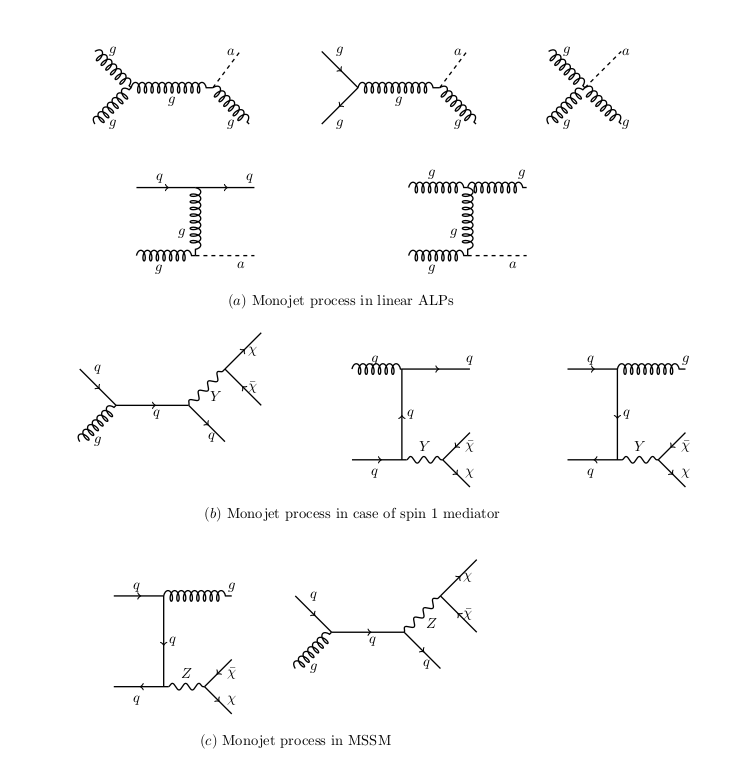
\includegraphics[scale=0.5]{figures/fyndiag.png}
\caption{Feynman diagrams for monojet process in the linear ALP (top), EFT framework with a massive spin-1 mediator (middle) and SUSY WIMP DM cases (bottom).\label{fyndiag}}
\end{figure*}
%%%%%%%%%%%%%%%%%%%%%%%%%%%%%%%%%%%%%%%%%%
\section{Description of Benchmark Models \label{sec:models}}
%%%%%%%%%%%%%%%%%%%%%%%%%%%%%%%%%%%%%%%%%%
In this section we describe our choices of benchmark models. These models span a large enough range of kinematic features to compare with SM processes, as well as to see the strength and limitations of the task of disentangling different DM scenarios.

\vspace{.5cm}
\begin{center}
\begin{tabular}{ c | c | c }\label{tab:bench}  Model & Mass & Type of coupling \\
\hline     SUSY1  & $m_{\tilde\chi^0}$= 100 GeV & Bino-like  \\
     SUSY2 & $m_{\tilde\chi^0}$= 200 GeV & Bino-like\\
     SUSY3 & $m_{\tilde\chi^0}$= 300 GeV & Bino-like  \\ \hline 
     ALP & negligible &  gluon-ALP \\ \hline
     EFT & negligible & 4-fermion \\ \hline
     
\end{tabular}
%\caption{Summary of benchmark models.}
\end{center}
\vspace{.5cm}

We first consider a set of three benchmarks in the WIMP DM scenario based on Bino-like SUSY neutralinos and with masses in the range 100 to 300 GeV, see Table~\ref{tab:bench}. We did not consider heavier WIMPs as they would likely be very hard to find at the LHC in monojet events. The cross section of production in monojet final states decreases quickly with the WIMP mass~\cite{Barducci:2015ffa}. 



To contrast against the WIMP we consider two alternative cases. The first is an Axion-Like Particle (or ALP) which is a paradigm for signatures from pseudo-Goldstone bosons. They can be light and collider-stable due to the derivative (suppressed) nature of their couplings. ALPs themselves could be a DM particle or can be a  DM mediator (see e.g. \cite{Lee:2012ph}). These exotic particles are constrained by Astrophysics as well as colliders in a complementary fashion~\cite{Mimasu:2014nea}. ALPs are also searched in axion experiments, which are designed to target their couplings with the photons. 

In this work, we do not restrict the ALP to be a DM candidate, and could decay after being produced, just not inside the detector~\footnote{If the ALP decays inside the detector, its detection would still be difficult due to its lightness. Nevertheless, one can still search for its effects on tails of distributions~\cite{Gavela:2019cmq}.}. It escapes detection as it has no charge under $SU(3)_c\times U(1)_Y$, hence its signatures are the same as DM, mono-searches. For the monojet channel, the  ALP relevant couplings are to gluons, as couplings to quarks are mass-suppressed: 
\begin{align}\label{eqn:L_eff}
    \mathcal{L}_a \supset 
 - \frac{g_{agg}}{2}a\,\text{Tr}\left[G_{\mu\nu}\tilde{G}^{\mu\nu}\right] . 
\end{align}
Note that the ALP-gluon coupling has the following bound \cite{Mimasu:2014nea,Brivio:2017ije}
\be g_{agg} \lesssim \unit[1.1\cdot10^{-5}]{GeV^{-1}} \quad (90\cl) \quad \text{for}\quad m_a \lesssim \unit[60]{MeV}\ee
Note that coupling of ALPs with photons or massive particles would lead to mono-photon, -W, -Z, -top and -Higgs signatures. 

We consider a second alternative scenario to WIMP DM based on light DM produced from the decay of the heavy mediator. We label this EFT DM, as the effective interaction between the SM and DM is via a four-fermion higher-order operator. The  simplified model Lagrangian which describes the interaction of DM ($\chi$) with the vector mediator ($Y$) is given by
\be  \mathcal{L}_{Y} =  \bar\chi \gamma_\mu g^V_{\chi} \chi Y^{\mu}.\ee and similarly for the interaction between the mediator and quarks. 
Note that the kinematic distribution of events is not very sensitive to the dark matter mass (see Fig. \ref{spin1med} in the appendix) in the limit of $m_Y \gg m_\chi$.  


Within these models, monojet signatures would result from the processes shown in Fig.~\ref{fyndiag}: a pair of DM particles (or a single ALP) produced in association with one initial state radiation (ISR) gluon or quark.   

Finally, we consider the dominant SM background given by $Z$+jets, where the $Z$ boson decays to neutrinos. 

%%%%%%%%%%%%%%%%%%%%%%%%
\section{Kinematic distributions\label{kinematics}}
%%%%%%%%%%%%%%%%%%%%%%%%

 
\begin{figure*}[t!]
\centering
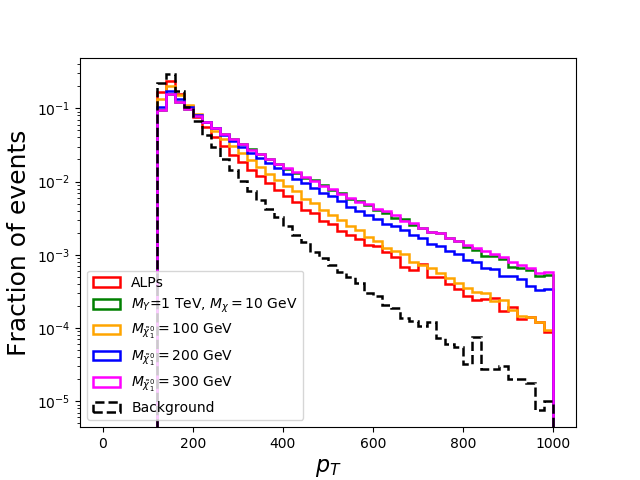
\includegraphics[scale=0.3]{figures/ptjallsb.png}
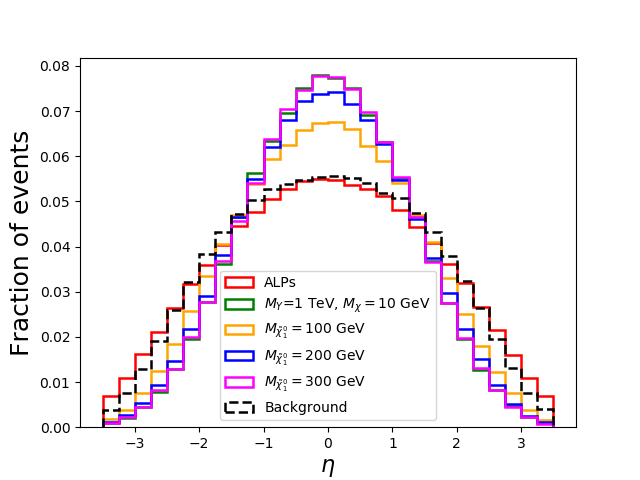
\includegraphics[scale=0.3]{figures/etajallsb.png}
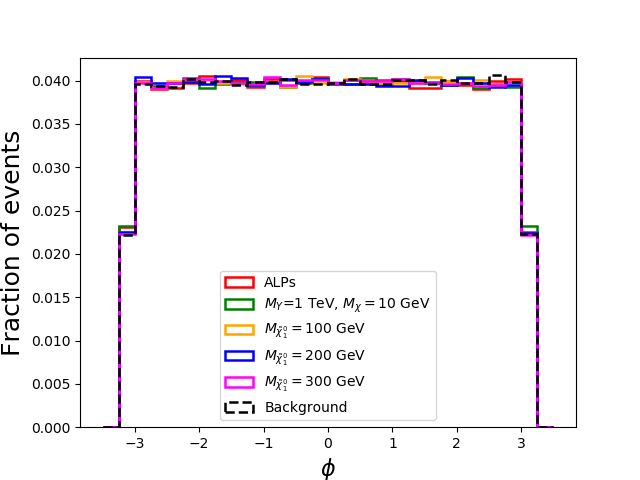
\includegraphics[scale=0.3]{figures/phijallsb.png}
\caption{Monojet parton-level LO 1D histograms for WIMP, EFT and ALP scenarios, as well as the SM background.\label{1DfeaturesPL1}}
\end{figure*}
\begin{figure*} [t!]
\centering
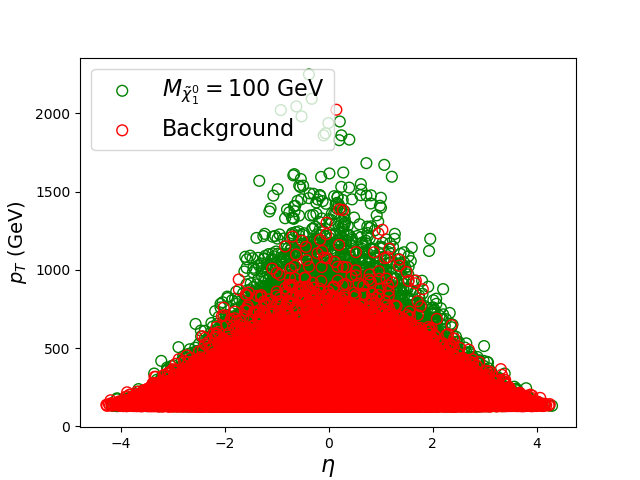
\includegraphics[scale=0.32]{figures/ptjetajsmsusy1.png}
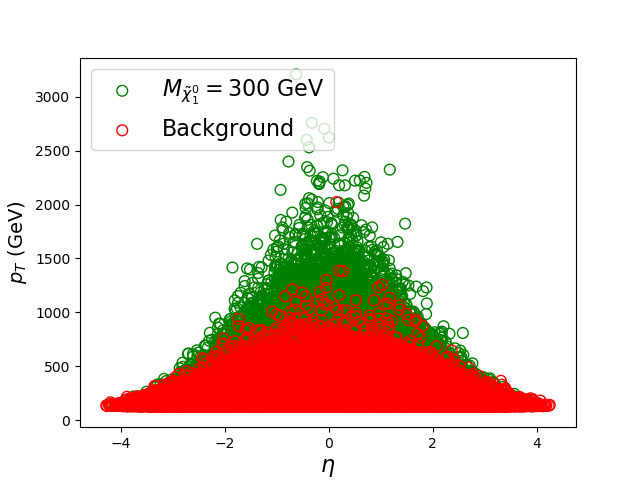
\includegraphics[scale=0.32]{figures/ptjetajsmsusy3.png}
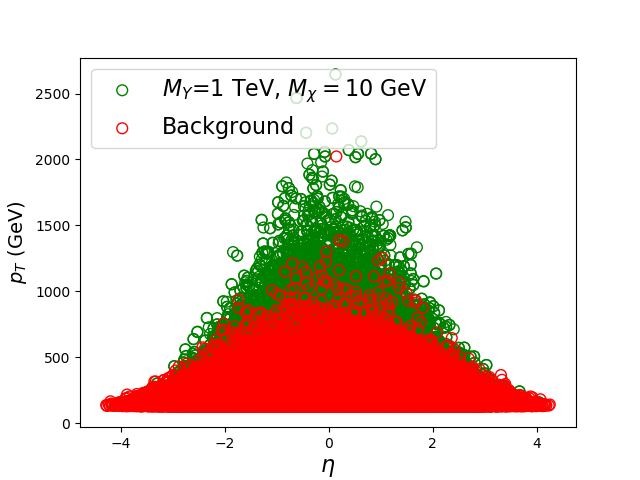
\includegraphics[scale=0.32]{figures/ptjetajsmeft.png}\\
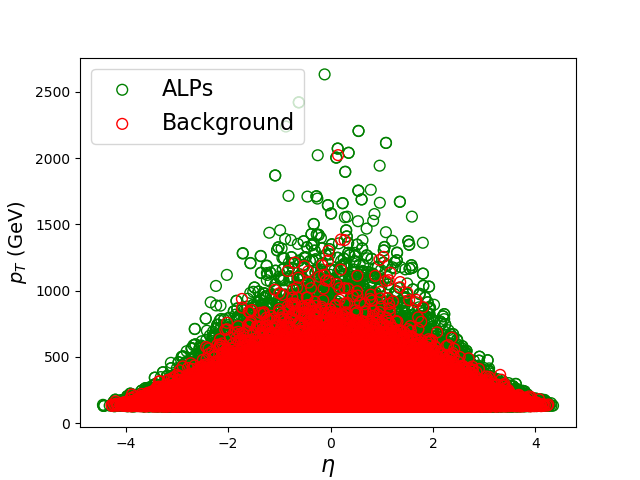
\includegraphics[scale=0.32]{figures/ptjetajsmaxion.png}
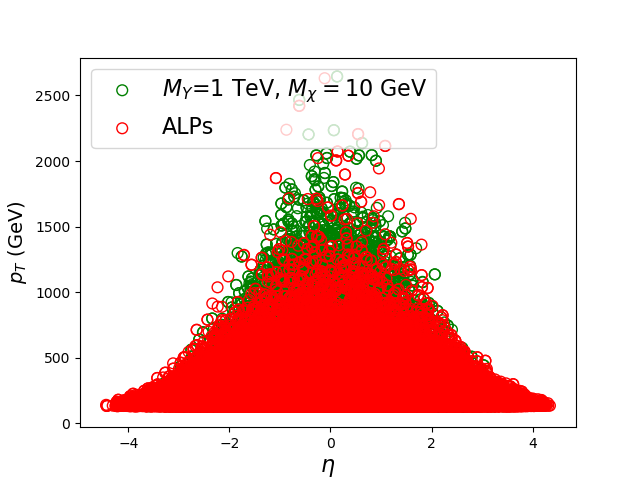
\includegraphics[scale=0.32]{figures/ptjetajaxspin1.png}
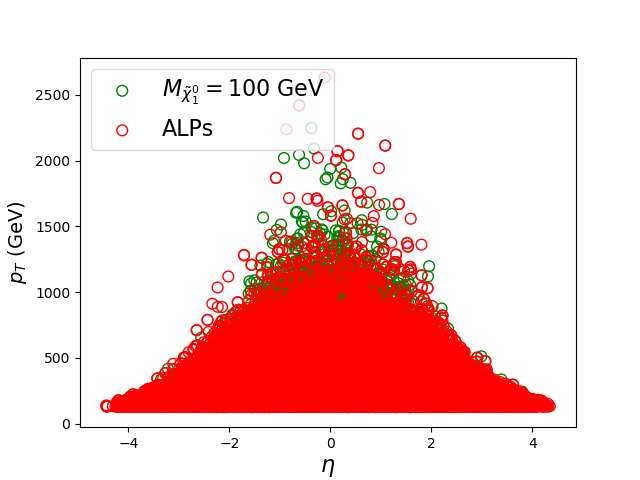
\includegraphics[scale=0.32]{figures/ptjetajaxsusy1.png}
\caption{Illustrative 2D histograms for the monojet final state at parton-level and LO in the plane of $p_T$ of the jet {\it vs} $\eta$. They are shown for several combinations of signals and signal  versus SM background.\label{1Dand2DfeaturesPL2}}
\end{figure*}
\begin{figure*}[t!]
\centering
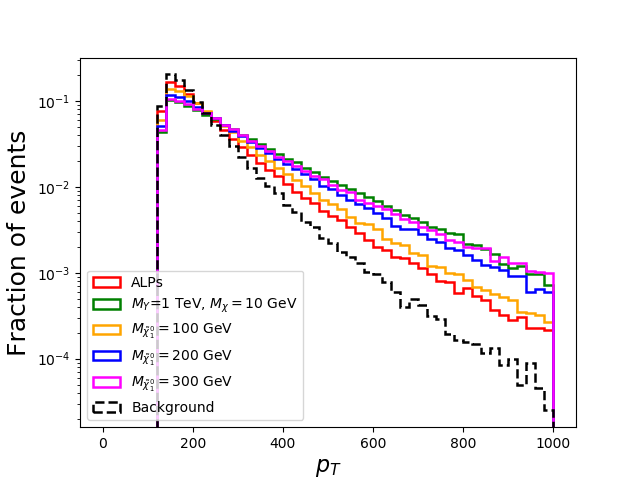
\includegraphics[scale=0.3]{figures/ptjallsbdelphes.png}
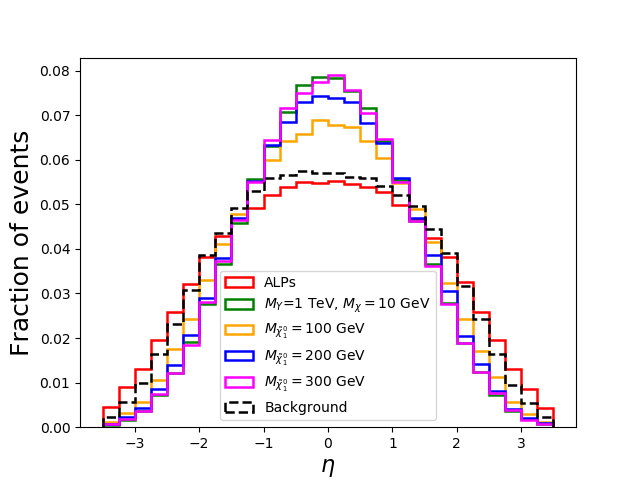
\includegraphics[scale=0.3]{figures/etajallsbdelphes.png}
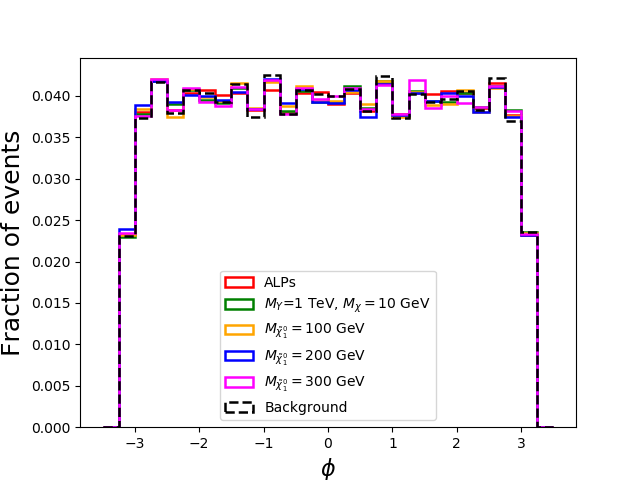
\includegraphics[scale=0.3]{figures/phijallsbdelphes.png}
\caption{Monojet detector-level 1D histograms for WIMP, EFT and ALP scenarios, as well as the SM background.\label{1Dand2DfeaturesDL}}
\end{figure*}
After presenting our benchmark scenarios for New Physics, in this section we describe the kinematic features which the Machine Learning algorithms will be able to optimize over. The aim of this section is to explain some of the features that the ML results will show.

The input for the ML studies is a list of events with their kinematic features simulated using a particular benchmark model.  We perform both parton- and detector-level simulations to generate the data samples. More details related to event generation
can be found in Appendix~\ref{setup}.

The kinematic features of those events are generically multi-dimensional, but one can project into 1D and 2D kinematic space. For example, in Fig.~\ref{1DfeaturesPL1} we show a set of 1D distributions for this process. Note that the jet transverse momentum in SUSY1 (lightest SUSY WIMP) and ALP is very similar, and also close to the  SM background distribution, whereas the other SUSY scenarios and the EFT exhibit a harder spectrum and easier discrimination with respect to the SM. Additionally, the pseudorapidity $\eta$ distribution of the jet is very similar for the ALP and SM background cases. 

At the level of 1D distributions, one cannot distinguish any preferred direction of the azimuthal angle $\phi$ distribution for both the New Physics signals and SM background processes.
\begin{figure*}[t!]
\centering
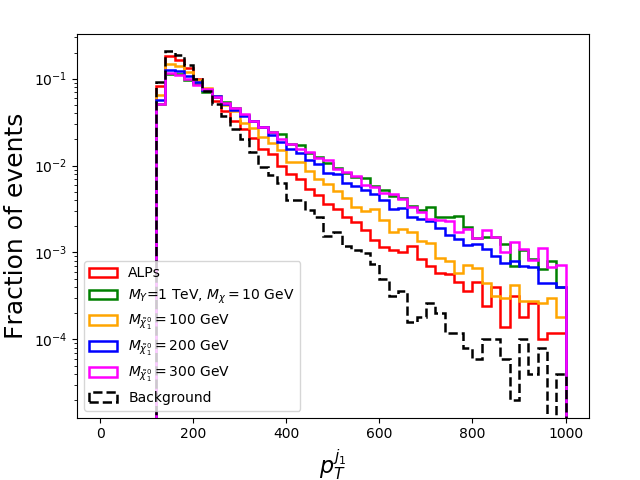
\includegraphics[scale=0.4]{figures/ptj1allsbdelphesdijet.png}
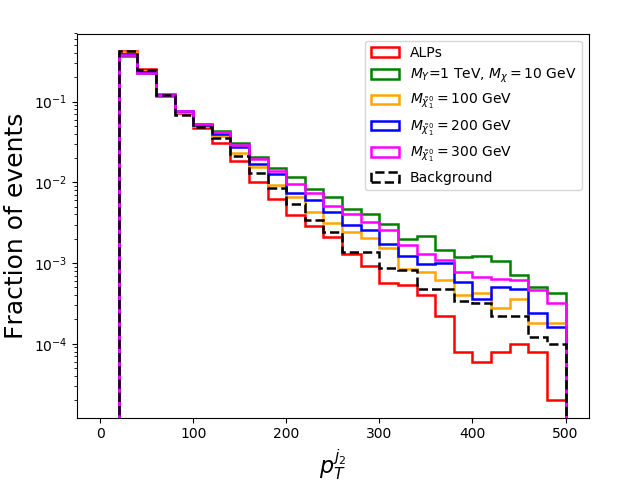
\includegraphics[scale=0.4]{figures/ptj2allsbdelphesdijet.png}\\
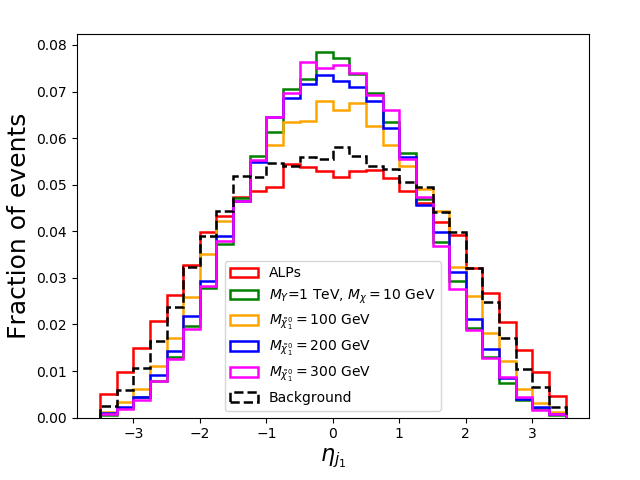
\includegraphics[scale=0.4]{figures/etaj1allsbdelphesdijet.png}
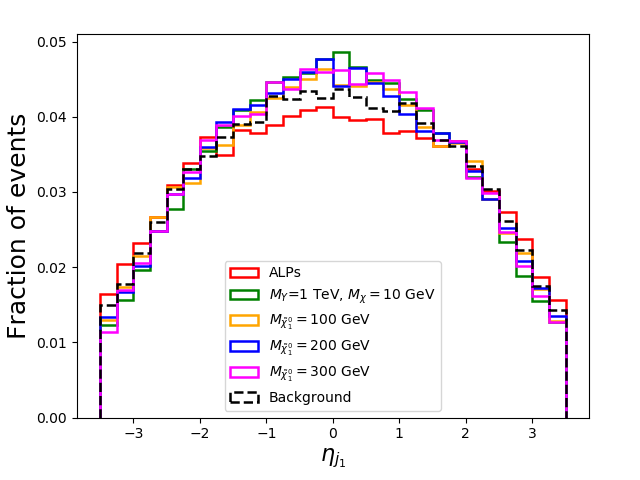
\includegraphics[scale=0.4]{figures/etaj2allsbdelphesdijet.png}\\
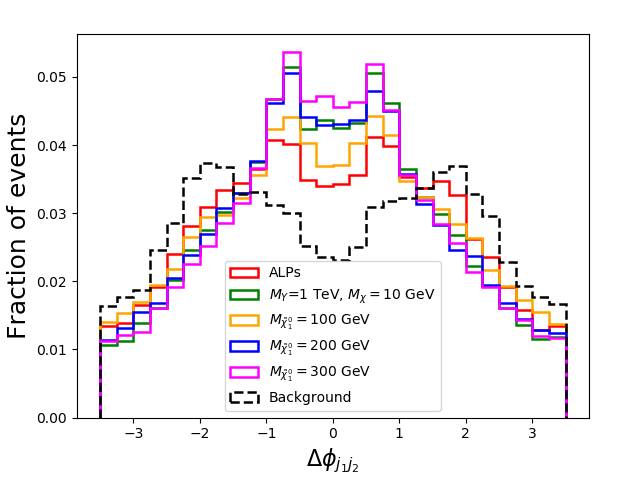
\includegraphics[scale=0.4]{figures/deltaphij1j2allsbdelphesdijet.png}
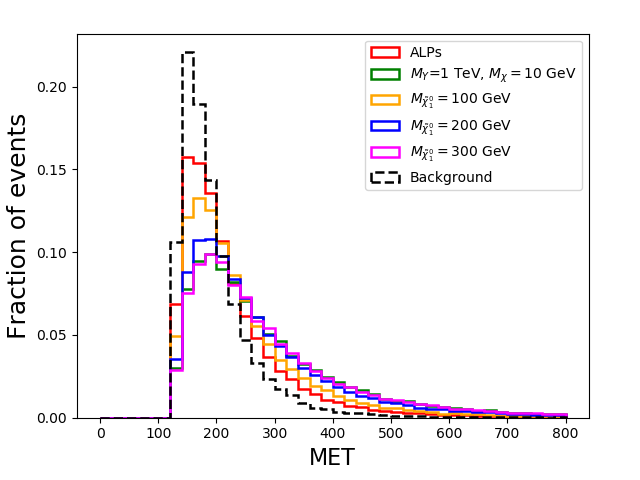
\includegraphics[scale=0.4]{figures/METallsbdelphesdijet.png}\\
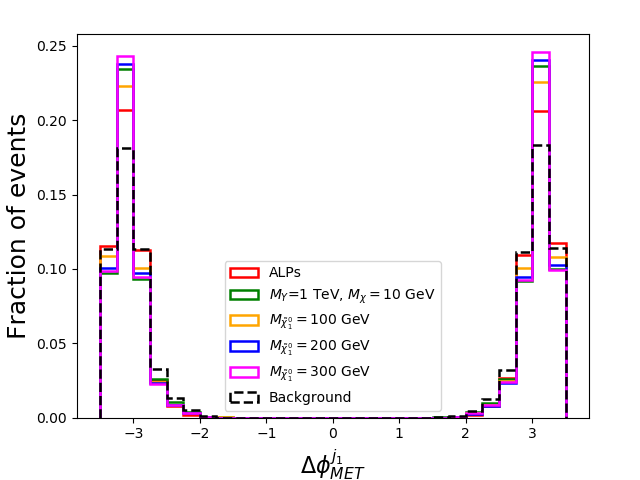
\includegraphics[scale=0.4]{figures/deltaphiMETj1allsbdelphesdijet.png}
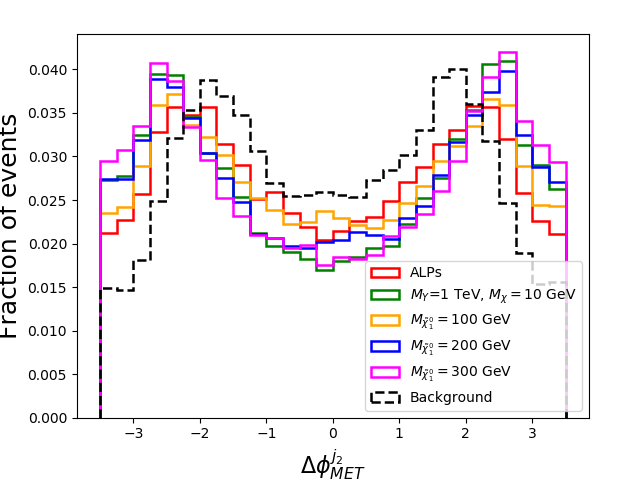
\includegraphics[scale=0.4]{figures/deltaphiMETj2allsbdelphesdijet.png}
\caption{Detector-level 1D histograms for the dijet process for WIMP, EFT and ALP scenarios, as well as the SM background.\label{1Dand2DfeaturesDLdijet}}
\end{figure*}
Additional information can be obtained when moving from 1D to 2D distributions, as shown in Fig.~\ref{1Dand2DfeaturesPL2} and discussed (in the Bayesian context) in Ref.~\cite{2D}, where we show the event distribution in the 2D plane of $p_T^j$ {\it vs} $\eta$. Different models are compared to each other in this plane. The top three panels show a clear difference in the high-$p_T$ region of SUSY1, SUSY3 and EFT benchmarks against the SM background. In the lower-leftmost plot we show that this is not the case for ALPs, whose $p_T$ distributions are not so peaked. Nevertheless, the $\eta $ and $p_T$ information is still useful. Finally, the two other lower plots show ALPs as compared to the EFT benchmark and the light SUSY case. The EFT case leads to harder $p_T$ spectrum and easier to differentiate from ALPs than the light SUSY case. We will see how the ML techniques will exhibit a similar trend. ALPs will be hard to separate from SUSY1, or light DM, whereas EFT and SUSY3 will have the most overlap, as both exhibit similar hard spectra. 


The characteristics of these rough features, broadening in pseudorapidity and $p_T$ reach, and what conclusions one can draw from them, depend on level of accuracy of our simulation. To explore robustness against showering and detector effects, we promoted the simulation to the {\tt Pythia} and {\tt Delphes} level. In Fig.~\ref{1Dand2DfeaturesDL} we show the same choices distributions as in Fig.~\ref{1Dand2DfeaturesPL2} but now at detector-level. The overall behaviour is indeed maintained from parton- to detector-level. 



Finally, we discuss how one would use another source of information from these monojet topologies. Monojet events do often contain an additional hard jet. Splitting or additional ISR emission is not extremely rare, and  with an additional object in the final state more information can be extracted of the DM nature. To account for the additional jet, we simulate detector-level events for the monojet (LO) and dijet (NLO) production. For all the cases, we consider data samples of 50K events with one additional
jet of $p_T>$ 25 GeV. 1D histograms for the constructed kinematic variable are shown in Fig. \ref{1Dand2DfeaturesDLdijet}. An additional jet provides a new source of kinematic information, enhancing the discriminating power of our study.  For example, notice that the distributions of $\Delta \phi_{j_1j_2}$ ($j_1$: leading jet, $j_2$: sub-leading jet) and 
 $\Delta \phi_{MET}^{j_2}$ are quite characteristic for the signals and background.

%%%%%%%%%%%%%%%%%%%%%%%%
\section{DM signal detection using Machine Learning\label{DMvsSM}}
%%%%%%%%%%%%%%%%%%%%%%%%

In this section we start our discussion on the  use of supervised Machine Learning techniques for Dark Matter signal classification. 

The input data we used for the analysis consists of three kinematic features of the monojet i.e. $p_T$, $\eta_j$ and $\phi_j$. We use this data both as an array input and also in the form of 2D histograms to build a ML algorithm. 

In the following sections, we will compare the performance of different methods, and also parton-level versus detector-level simulations. For this analysis, we will consider the kinematics of the leading jet ($p_T>130$ GeV) for the LO analysis and in addition to this also of the sub-leading jet for the NLO data sample. For the reasons mentioned in Sec.~\ref{sec:models}, we do not use the cross-section information,   so a balanced dataset is considered for all the classes. Data samples are divided in 70$\%$ $:$ 30$\%$ proportions for the training and test samples. 
%%%%%%%%%%%%%%%%%%%
\subsection{Logistic Regression}
%%%%%%%%%%%%%%%%%%%
At first step, we perform logistic regression for the monojet data in the form of arrays. 

We used SGDclassifier of \textsc{sklearn} python library with a log-loss function.  For the parton-level events, Receiver operating characteristic (ROC) curves for all the signals are shown in Fig. \ref{rocLO-LR}. We can see that the value AUC\footnote{AUC (area under the ROC curve) is a measure of the algorithm's performance.} varies from 0.58 to 0.71 for the ALP and SUSY3 case, and the other three cases lie in-between. In other words, one can {\it easily} separate heavy WIMPs from the Z$+$jet SM background, however ALP monojet would not be efficiently classified. The regularization parameter $\lambda= 10^{-5}$ is used for all the cases.
\begin{figure}[h!]
\centering
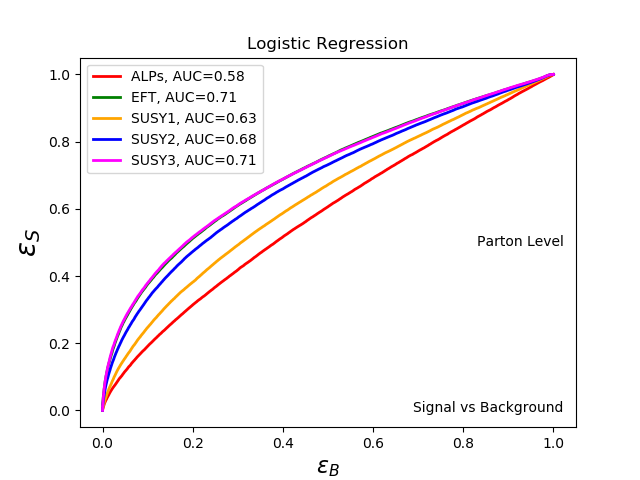
\includegraphics[scale=0.50]{figures/ROCsbLR.png}
\caption{ROC curves using logistic regression for different signals versus background for the LO parton-level analysis.}\label{rocLO-LR}
\end{figure}

%%%%%%%%%%%%%
\subsection{Neural Networks-kinematic features}
%%%%%%%%%%%%%
\begin{figure}%[h!]
\centering
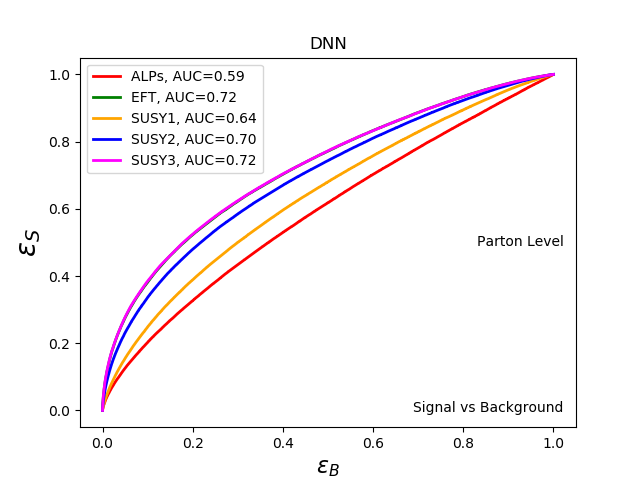
\includegraphics[scale=0.50]{figures/ROCsbNN.png}
\caption{ROC curves using Neural Networks   for different signals versus background for the LO parton-level analysis. 
}\label{rocLO-NN}
\end{figure}
\begin{figure}% [h!]
\centering
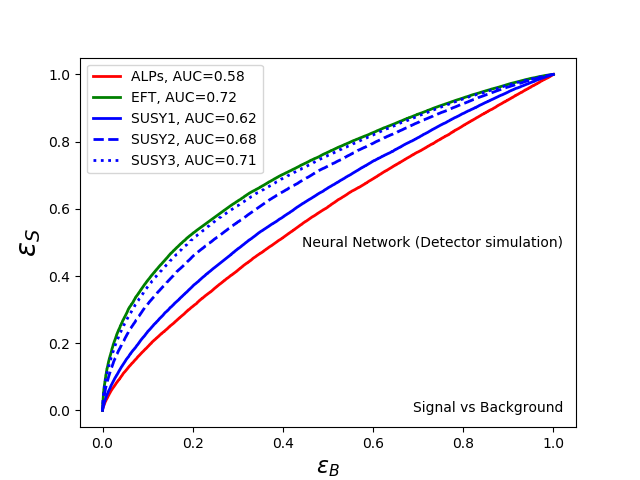
\includegraphics[scale=0.50]{figures/ROCsbNNdelphes.png}
\caption{ROC curves using Neural Networks for different signals versus background for the LO detector-level simulated data. 
 }\label{roc-LOdelphes-NN}
\end{figure}
We investigate the classification accuracy using Deep Neural Networks (DNN) with the same input features
i.e. $p_T$, $\eta$ and $\phi$ of the jet. We used five fully-connected hidden layers for the network as including more layers
does did improve the performance. 

For all the layers, except the final one, the number of neurons equal to the number of data features that are considered. 
For the intermediate layers, a {\tt ReLU} activation function is used, whereas we use a `sigmoid' function  for the output layer. We considered the binary cross-entropy loss function. The `dropouts'  option is also activated, with 0.2 as the optimized choice. Finally, the `adadelta' optimizer, and  batch-size and epochs are set to 500 and 300, respectively. 

In Fig.~\ref{rocLO-NN}  we show the ROC curves for various signals at parton-level, whereas the classification accuracy for the detector-level event generation is shown in figure \ref{roc-LOdelphes-NN}. The DNN is able to classify signal versus background at a very similar level as a logistic regression algorithm, only marginally better. As in the previous sub-section, ALPs are more difficult to pick up from the SM background, a task that becomes simpler and simpler as we increase the mass of the DM particle. SUSY3 and EFT, as expected, exhibit very similar performances, and in Fig.~\ref{rocLO-NN} the two lines overlap each other. 
\begin{figure} %[h!]
\centering
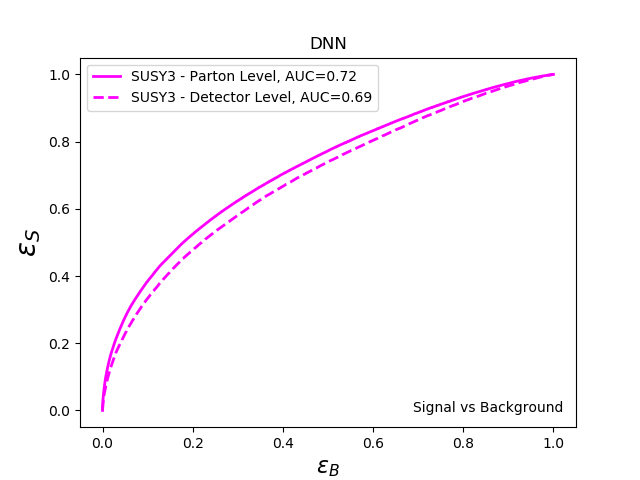
\includegraphics[scale=0.50]{figures/ROCsbNNcomparePLandDelphes.png}
\caption{Comparison of DNN ROC curves  for WIMP SUSY3 versus background for parton-level and detector-level simulations.}\label{roc-LO-PL-delphes-NN}
\end{figure}

To finish this section using DNNs with the three kinematic inputs, we discuss some aspects of the analysis. 


The first aspect relates to the robustness of the analysis with changes in the level of simulation detail. In Fig.~\ref{roc-LO-PL-delphes-NN}, we compare
the ROC curves for parton- and detector-level data samples for the SUSY3 versus SM background case. The difference in both cases is very small, indicating that the DNN classification efforts are robust. 

We also compared the performance of DNNs  with just two variables (by excluding the $\phi$ variable) and found that there is no degradation in the classification accuracy. This is expected, as the three input variables are redundant once energy-momentum conservation within the event is taken into account. 
\begin{figure}% [h!]
\centering
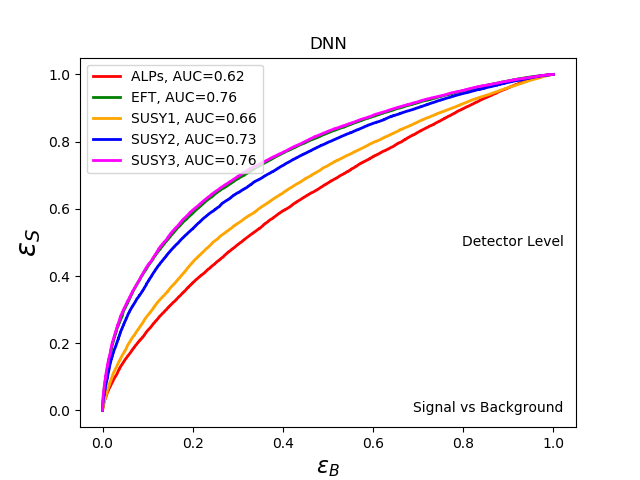
\includegraphics[scale=0.50]{figures/ROCsbNNdelphesNLO.png}
\caption{NN NLO detector-level ROC curves for different signals versus background. 
 }\label{roc-NLOdelphes-NN}
\end{figure}
Finally, we explore the benefit of considering  NLO dijet  processes in addition to monojet.  In this case we consider eight features: $p_T^{j_1}, p_T^{j_2}, \eta^{j_1}, \eta^{j_2}$, $\text{MET}$, $\Delta \phi_{j_1j_2}, 
\Delta \phi_{MET}^{j_1}$, and  $\Delta \phi_{MET}^{j_2}$. Using the DNN with the same architecture for this data sample we get indeed an enhancement in the classification accuracy as shown in Fig.~\ref{roc-NLOdelphes-NN}.




%%%%%%%%%%%%
\subsection{DNN with 2D histograms}
%%%%%%%%%%

As mentioned earlier, the information in the monojet event is saturated by choosing two variables, e.g. $p_T^j$ and $\eta^j$. Therefore, inspired by the use of Convolutional Neural Networks (CNNs) in the classification of images, we construct `images' from 2D histograms using $p_T$ and $\eta$ of the jet. 

\begin{figure*}%[h!]
\centering
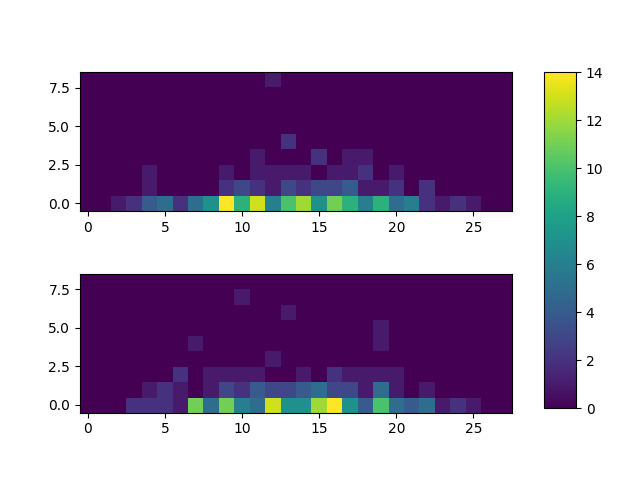
\includegraphics[scale=0.32]{figures/picsusybp1200eventscombo.png}
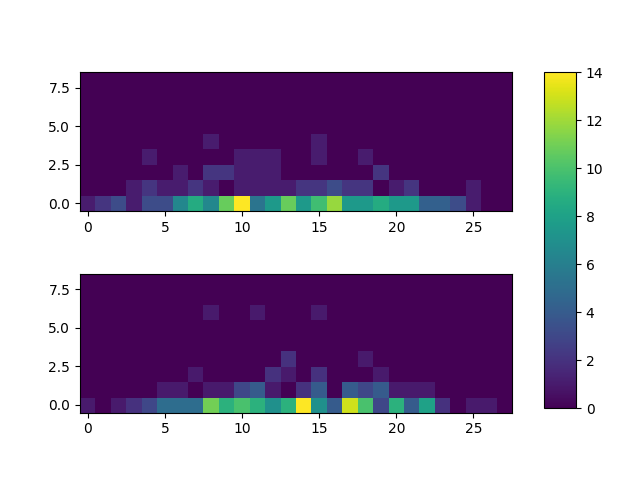
\includegraphics[scale=0.32]{figures/picaxion200eventscombo.png}
\caption{Illustrative 2D histograms for SUSY1 (left) and ALP case (right) averaging over 200 events.}\label{demopic}
\end{figure*}

One has choices on how to group the events into images. The simulated dataset  contains $N_\text{Tot}$ total number of events, and is divided into $N_\text{Images}$ number of images, such that each image contains $r=N_\text{Tot}/N_\text{Images}$ number of events. 

 Creating a number of `images' to train a network  is a powerful tool since each image is itself giving an approximation of the joint Probability Density Function (PDF) distribution for both $p_T$ and $\eta$. The degree to which each image approximates the PDF depends on the number of events $r$ chosen to be in an image. For a fixed total number of events (integrated luminosity) there will then be a trade-off between $r$ and $N_\text{Images}$ that will affect the accuracy of the model.


\subsubsection{Monojet-LO}
Before analysing the data with a CNN, we first attempt solving the problem with a DNN. This is achieved by decomposing the 2D histogram into a 1D array with values corresponding to the normalised number of events in each bin. Note that whilst the may seem like we are just reconstructing the original distributions, this is not the case since this data now contains correlations from individual distributions. A few illustrative pictures of these plots are shown in Fig.~\ref{demopic}.

We consider $p_T$ and $\eta$ in range [130, 2000] GeV and [-4 to 4], respectively with 29 $\times$ 29 bins. We use the information of event density in this grid as an input for a DNN. The network is well optimised with two fully connected hidden layers, both consisting of twenty neurons with a {\tt ReLU} activation function and a {\it softmax} activation function for the output layer. After investigation, we do not find over-training to be an issue, so only include a small number of dropout neurons. The network is trained for 300 epochs with a batch size of 500. We evaluate the network's performance through accuracy (found from finding whether the predicted result (ranging from 0 to 1) round to 0 or to 1). This is done within the training dataset whilst training, then with the validation dataset whilst evaluating how the network is training, and finally with the test dataset. The ROC curves for signal to background identification using DNNs with the 2D histograms for $r=20$ are shown in Fig. \ref{2D_DNN_sig_vs_bg_LO_ROC}. 

We find yet again that the differences between the classification accuracies for the parton- and detector-level events is not significant. 

\begin{figure}% [H]
\centering
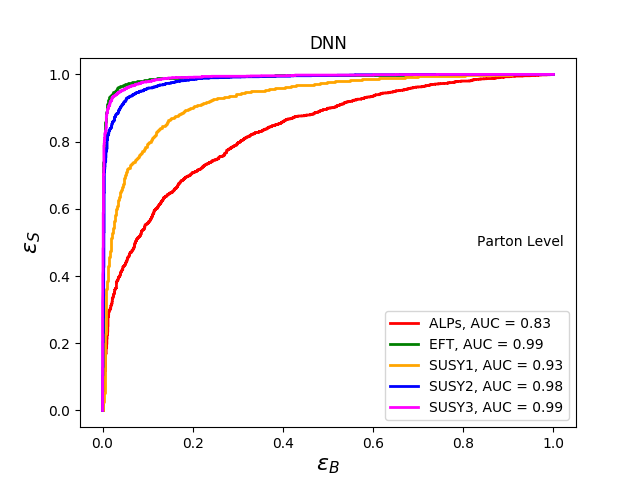
\includegraphics[scale=0.50]{figures/2D_DNN_sig_vs_bg_LO_ROC.png}
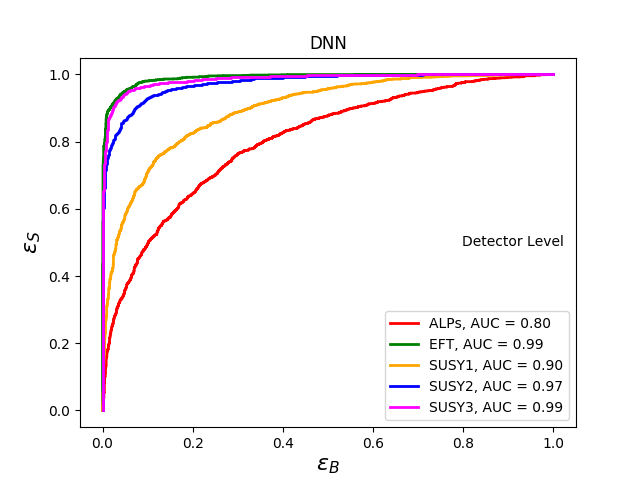
\includegraphics[scale=0.50]{figures/2D_DNN_sig_vs_bg_delphes_ROC.png}
\caption{ROC curves (DNN with 2D histograms, $r = 20$) for signal versus background for the parton-level (upper) and detector-level (lower) simulations. For these plots, 200K events were used.}\label{2D_DNN_sig_vs_bg_LO_ROC}
\end{figure}


\subsubsection{Monojet-NLO}
We also consider the Next-to-Leading-Order (NLO) processes in which two parton-level jets in addition to the 1-jet process are produced. We also simulate detector-level for the NLO processes, and use both the leading jet as well as the jet with the second highest transverse momentum. More details about how two jet events are selected can be found in the Appendix~\ref{setup}. 

Since for the NLO process we have eight different features, there are 28 possible variations of 2D histograms that we could produce. If this were to be fully taken into account, then it might prove fruitful to combine the results of those 28 ML algorithms together in some manner. Alternatively, one could produce three (or higher)-dimensional histograms and deconvolve them for the DNN, or use a three (or higher)-dimensional CNN. However, we shall not take this approach here to avoid the risk of over-complicating an analysis which may not benefit from it and obscure the physics. Instead, we perform a Principal Component Analysis (PCA) to the NLO data in order to determine which features are more relevant.

\begin{figure}% [H]
\centering
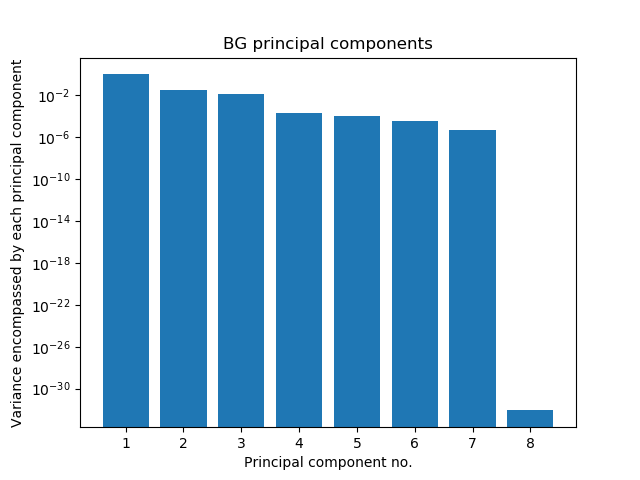
\includegraphics[scale=0.26]{figures/BG_PCA.png}
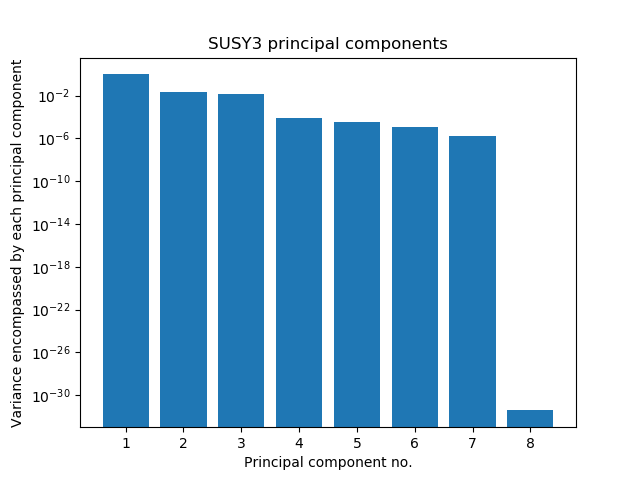
\includegraphics[scale=0.26]{figures/SUSY3_PCA.png}
\caption{The explained variance ratio of the new principal component axes (with the number of principal component axes being 8, the same number of original features), highlighting the relative importance of the principal components in terms of capturing variance in the datasets.}\label{PCA_plots1}
\end{figure}
Figure~\ref{PCA_plots1} (and Fig.~\ref{PCA_plots2} in the Appendix) shows that whilst all but one feature columns contribute to the variance of the dataset, a significant amount of the variance within the datasets is captured
within the first three principal component axes. By finding the correlation between the original features and the new principal component axes, we can determine which features are most important in terms of holding information. We expect an increase in classification performance if we were to use the principal component axes as new feature columns, however we choose instead to use the original feature columns that correspond most strongly to the most important principal component axes, as we are primarily interested in establishing which features are most relevant for our 2D analysis as a proof-of-concept. 

The correlations can be seen in Table~\ref{PCA_table1} for the SM background and the SUSY3 benchmark, and for other cases in Tables \ref{PCA_table2}, \ref{PCA_table3}, \ref{PCA_table4}, and \ref{PCA_table5} of the Appendix~\ref{PCA}. 

One can see from the table that the three most important features are the same for all datasets, namely  $p_T^{j_1}$, $\Delta \phi_{j_1j_2}$, and $\Delta \phi_{\text{MET}}^{j_1}$.


\begin{table}
\centering
\scalebox{0.95}{
\begin{tabular}{|c|c|c|c|c|c|c|c|c|}
\hline
\multicolumn{9}{|c|}{Background PCA correlations} \\
\hline
\toprule
{} &  $p_T^{j_1}$ &  $p_T^{j_2}$ &  $\eta_{j_1}$ &  $\eta_{j_2}$ &  $\Delta \phi_{j_1j_2}$ &   $\text{MET}$ &  $\Delta \phi_{\text{MET}}^{j_1}$ &  $\Delta \phi_{\text{MET}}^{j_2}$ \\ \hline
\midrule
PC-1 &  0.67 &  0.41 &  -0.01 &  -0.01 &  -0.01 &  0.62 &      0.00 &     -0.00 \\ \hline
PC-2 &  0.00 &  0.00 &   0.01 &   0.00 &   0.45 & -0.00 &     -0.77 &     -0.45 \\ \hline
PC-3 & -0.00 & -0.00 &   0.09 &   0.10 &  -0.70 & -0.00 &      0.00 &     -0.70 \\ \hline
PC-4 & -0.01 &  0.00 &  -0.70 &  -0.70 &  -0.09 & -0.01 &     -0.01 &     -0.10 \\ \hline
PC-5 & -0.12 &  0.89 &  -0.01 &   0.02 &  -0.00 & -0.45 &      0.00 &      0.00 \\ \hline
PC-6 & -0.01 &  0.01 &   0.71 &  -0.71 &  -0.01 & -0.01 &      0.01 &     -0.00 \\ \hline
PC-7 &  0.73 & -0.23 &   0.00 &   0.00 &   0.00 & -0.65 &      0.00 &      0.00 \\ \hline
PC-8 &  0.00 &  0.00 &  -0.00 &  -0.00 &   0.54 & -0.00 &      0.64 &     -0.54 \\ \hline
\bottomrule
\end{tabular}}
%\end{table}
%\begin{table}
\scalebox{0.95}{
\begin{tabular}{|c|c|c|c|c|c|c|c|c|}
\hline
\multicolumn{9}{|c|}{SUSY3, $M_{\tilde{\chi}_1^0} = 300$ GeV PCA correlations} \\
\hline
\toprule
{} &  $p_T^{j_1}$ &  $p_T^{j_2}$ &  $\eta_{j_1}$ &  $\eta_{j_2}$ &  $\Delta \phi_{j_1j_2}$ &   $\text{MET}$ &  $\Delta \phi_{\text{MET}}^{j_1}$ &  $\Delta \phi_{\text{MET}}^{j_2}$ \\ \hline
\midrule
PC-1 &  0.67 &  0.32 &   0.00 &   0.01 &   0.00 &  0.67 &     -0.00 &     -0.00 \\ \hline
PC-2 & -0.00 & -0.01 &   0.01 &  -0.01 &   0.32 & -0.00 &     -0.76 &     -0.57 \\ \hline
PC-3 &  0.00 & -0.00 &  -0.07 &  -0.06 &  -0.80 &  0.00 &      0.11 &     -0.58 \\ \hline
PC-4 & -0.01 &  0.02 &   0.70 &   0.70 &  -0.07 & -0.01 &      0.01 &     -0.05 \\ \hline
PC-5 & -0.22 &  0.95 &  -0.00 &  -0.02 &   0.00 & -0.23 &     -0.01 &     -0.00 \\ \hline
PC-6 & -0.00 &  0.01 &  -0.71 &   0.71 &   0.01 & -0.00 &     -0.01 &     -0.00 \\ \hline
PC-7 &  0.71 & -0.01 &  -0.00 &   0.00 &  -0.00 & -0.71 &      0.00 &      0.00 \\ \hline
PC-8 &  0.00 &  0.00 &   0.00 &  -0.00 &   0.50 &  0.00 &      0.64 &     -0.58 \\ \hline
\bottomrule
\end{tabular}}
\caption{PCA original feature to principal component correlations for the SM background and SUSY3 (rounded to 2 d.p.).}\label{PCA_table1}
\end{table}

\begin{figure}% [H]
\centering
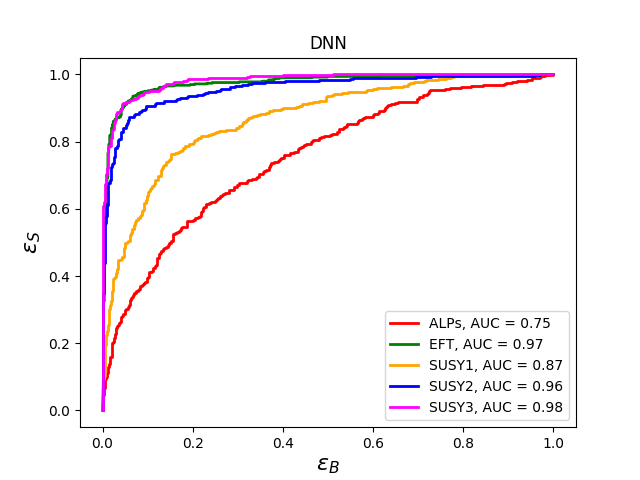
\includegraphics[scale=0.50]{figures/2D_DNN_sig_vs_bg_delphes_pt-metphij1_ROC.png}
\caption{ROC curves (DNN with 2D histograms, $r = 20$) for signal versus background for the dijet NLO detector level simulation with 50K event samples.}\label{2D_DNN_sig_vs_bg_NLO_ROC}
\end{figure}


In the following we shall use $p_T^{j_1}$ and $\Delta \phi_{\text{MET}}^{j_1}$ to construct 2D histograms since they are the two features which occur the most amongst the top two principal components. However, one should be able to gain from including the other features as well. We do find an increase in classifier performance when using these two distributions over $p_T^{j_1}$ and $\eta_{j_1}$. The ROC curves for a DNN (with the same architecture as before) are shown in Fig. \ref{2D_DNN_sig_vs_bg_NLO_ROC} (signal-to-background).

For comparison, we use the same  most informative combinations among different cases, namely SUSY WIMP versus other benchmarks.   If we compare this case with the LO case (Fig. \ref{2D_DNN_sig_vs_bg_LO_ROC}), the NLO AUC is smaller than LO value for signals which look more like SM, i.e. ALP and SUSY1. This is a manifestation that  the  NLO full event information is confined in more than two kinematical variables and we are not exploiting the full available information. As mentioned earlier, the same could be done by using the PCA components.

\subsection{CNN with 2D histograms}
After transforming our events into images, approximations of PDFs, and processing them using a DNN, we move onto applying CNNs to them.  

We use a CNN with two convolutional layers, two max-pooling layers and one dense 
flatten hidden layer, with {\tt ReLu} activation function for all the cases.

The ROC curves for all the signals versus SM background are shown in Fig. \ref{2D_CNN_sig_vs_bg_LO_ROC}. As mentioned earlier, CNNs are able to retain the information of spatial correlations and usually perform better than DNNs for the image data. But in our case, because images are constructed from highly processed information (PDFs are already an abstract concept) we find no sizeable improvement respect to the DNN results. The corresponding  ROC curves are shown in Fig. \ref{2D_CNN_sig_vs_bg_NLO_ROC} for the NLO case. The performance for the LO (detector-level) and NLO data sample is the same and is lower than the parton-level LO analysis for the ALPs and SUSY1 case. 


\begin{figure}% [H]
\centering
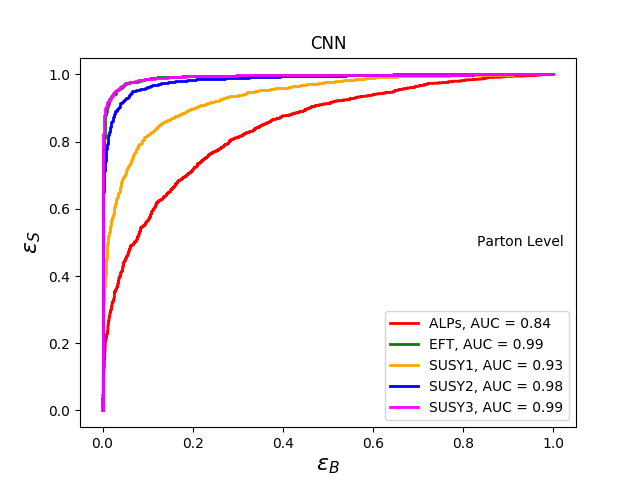
\includegraphics[scale=0.50]{figures/2D_CNN_sig_vs_bg_LO_ROC.png}
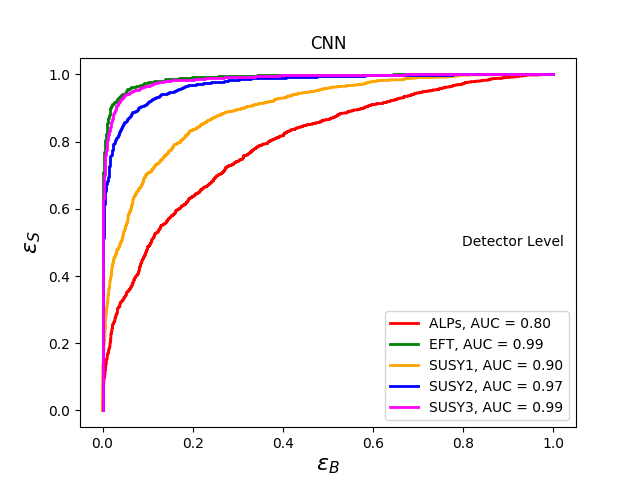
\includegraphics[scale=0.50]{figures/2D_CNN_sig_vs_bg_delphes_ROC.png}
\caption{ROC curves (CNN with 2D histograms, $r = 20$) for signal versus background for the parton-level (upper) and detector-level simulation (lower). For these plots, 200K events are used for each process in both the cases.}\label{2D_CNN_sig_vs_bg_LO_ROC}
\end{figure}




\begin{figure}% [H]
\centering
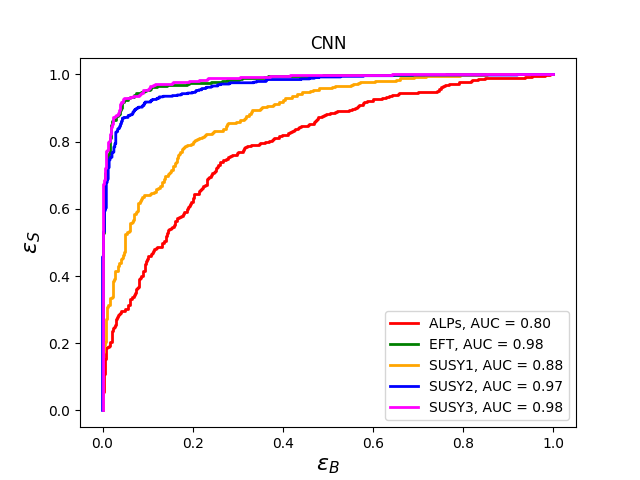
\includegraphics[scale=0.50]{figures/2D_CNN_sig_vs_bg_delphes_pt-metphij1_ROC.png}
\caption{ROC curves (CNN with 2D histograms, $r = 20$) for signal versus background for the dijet NLO detector level simulation. For these plots, 50K events are used for each process in both the cases.}\label{2D_CNN_sig_vs_bg_NLO_ROC}
\end{figure}


 
%%%%%%%%%%%%%%%
\section{DM Characterization\label{DMvsDM}}
%%%%%%%%%%%%%%%

In the previous section we discussed the identification of different monojet signals respect to the SM leading background. We found that heavy WIMPs and EFT monojet signals are easier
to distinguish from the SM background, as expected. But at the same time, these two benchmarks are quite similar to each other when compared with the SM. Nevertheless, the SUSY3 benchmark corresponds to a DM particle of 300 GeV, whereas the EFT corresponds to a DM particle with negligible mass. 

The next question arises, i.e. whether it is possible to disentangle an electroweak-scale WIMP DM signal from an ALP or an EFT signal with very light DM. 

We use NNs with kinematic features as input for the 
classification of different signals. As we have seen in the previous section, classification accuracy is not very different for the detector level simulated data, hence we consider parton-level data in this section. The architecture of NN is kept to be the  same as in the previous section. 

\begin{figure}% [H]
\centering
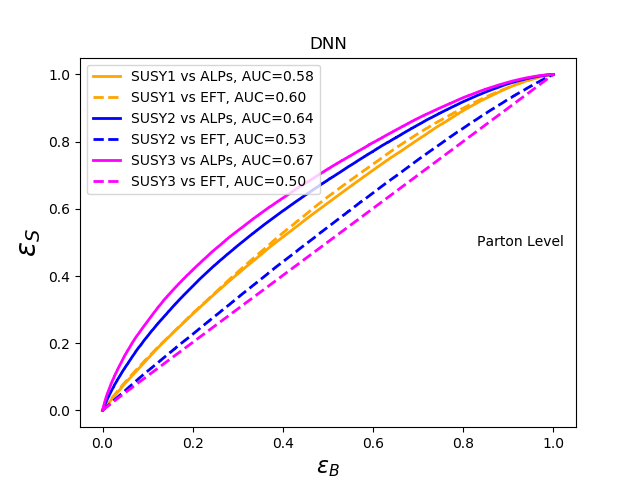
\includegraphics[scale=0.50]{figures/ROCssNN.png}
\caption{ROC curves using neural network for different WIMP scenarios versus ALP/EFT signals (LO parton-level analysis). 
}\label{result2}
\end{figure}

In Fig.~\ref{result2}, we show the ROC curves for the  WIMP signal, where the other new physics signals are taken as competitors. We consider the three benchmark values for
the neutralino mass in the WIMP scenario described in Sec.~\ref{sec:models}. ROC AUC for WIMP SUSY3 versus EFT, and SUSY1 versus axion signal are 0.50 and 0.58 respectively. Therefore the
likelihood to misidentifying light WIMPs and axions is very high, and the same is true for heavy WIMP and EFT DM. 



\begin{figure}% [H]
\centering
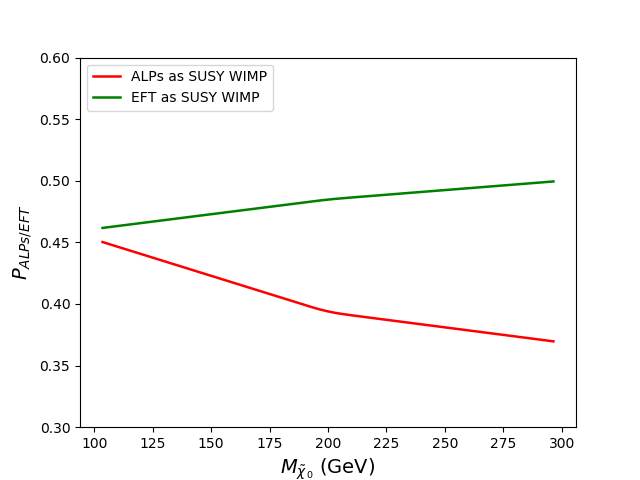
\includegraphics[scale=0.50]{figures/fprsusy-ALPeft.png}
\caption{Probability of misidentifying ALPs or EFT DM scenarios with a true SUSY WIMP as a function of the neutralino mass (parton-level LO data).}\label{result3}
\end{figure}

Another way to express this statement is shown in Fig.~\ref{result3}, where we plot the likelihood that a true WIMP signal is misidentified for an ALP or EFT DM scenario. The likelihood is computed as the false positive rate for the optimal point on the ROC curve. 

Since we are not considering the weight of the cross-section for different signals, we find the optimal point by minimizing the Euclidean distance from the (1=\textsc{TPR}\footnote{TPR is fraction of signal events correctly identified by the algorithm, and FPR is the fraction of background events identified as signal events by the algorithm.},0=\textsc{FPR}) value. 


For DM identification we also use 2D histograms of $p_T$ and $\eta$ of the jet. As discussed in the previous section for signal versus background, in this case  averaging over more number of events per image  improves the classification accuracy. As an illustration of this effect, in Fig. \ref{accuracy1}, we show the accuracy plot for WIMP SUSY3 versus ALPs data and how it depends on the number of events injected in one picture for the fixed data sample. The different colored curves correspond to varying the total data sample. For a fixed data sample, the number of images a  DNN is trained and tested is reduced when we increase the number of events per image. In Fig.~\ref{accuracy2}, we show the small data sample curves with the error bars. Note that these images  are feeding the NN a likelihood function to different degrees of approximation, depending on how many events per image are considered. 

We studied the dependence of the  accuracy with the size of the data sample. Once we have enough data to train the NN, adding more events does not improve accuracy, whereas the accuracy decreases for smaller values of `r'. The model becomes unstable for the 10K data sample. We ran the DNN code many times to get a band of accuracy. Using the total number of 100K data sample the DNN is very stable, but it starts becoming unstable for the 50K data sample. For the smaller `r' values, input images do not look very different and on top of this smaller data sample makes it difficult to get stable model parameters. In Fig.~\ref{accuracy1}, for the 50K, 20K and 10K data sample, central values of accuracy are plotted. For the 10K data sample (Fig.~\ref{accuracy2}), we see that the error is bigger for $r=20$ than $r=25$ value. This could also be the case due to the asymmetric error. For the further smaller data sample, DNN's performance completely collapses.

ROC curves for the signal-to-signal identification using DNN are shown in Figs.~\ref{2D_DNN_SUSY_vs_sig_LO_ROC}  and \ref{2D_DNN_SUSY_vs_sig_NLO_ROC}, for the LO and NLO data sample respectively. 

For the NLO sample, 2D histograms of $p_T^{j_1}$ and $\Delta \phi_{\text{MET}}^{J_1}$ are constructed as in the previous section. In this case also, we used CNNs and the ROC curves are shown in Figs.~\ref{2D_CNN_SUSY_vs_sig_LO_ROC}
and  \ref{2D_CNN_SUSY_vs_sig_NLO_ROC}, for LO and NLO processes respectively.




\begin{figure}% [H]
\centering
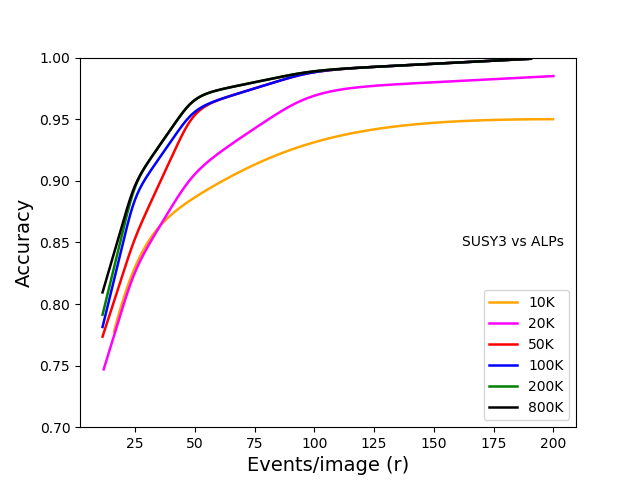
\includegraphics[scale=0.50]{figures/accuracyplot2dSUSY3vsAxion.png}
\caption{Accuracy versus number of events per image, with varying total number of events for SUSY3 versus ALP. We  use fully-connected NNs with two hidden layers for different data sample size. The parton-level data set is considered for this plot.} \label{accuracy1}
\end{figure}

 
\begin{figure}% [H]
\centering
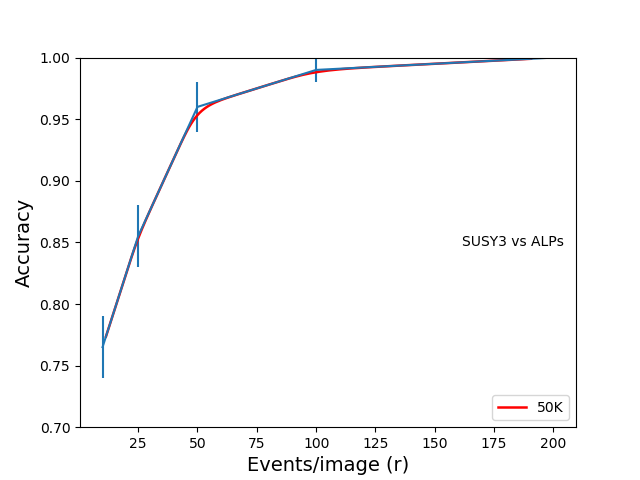
\includegraphics[scale=0.50]{figures/accuracyband2dSUSY3vsAxion50k.png}
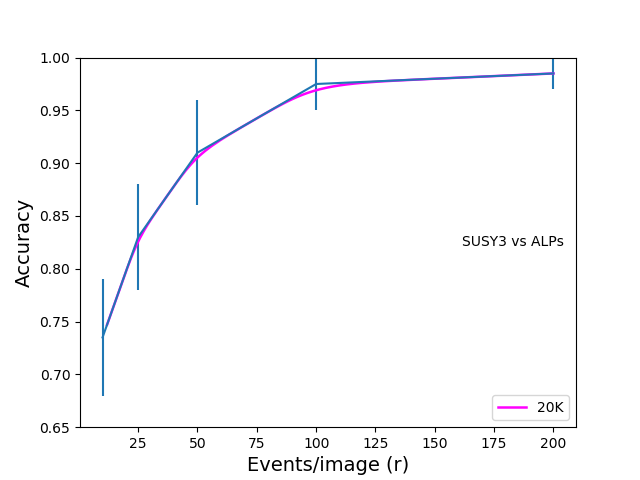
\includegraphics[scale=0.50]{figures/accuracyband2dSUSY3vsAxion20k.png}
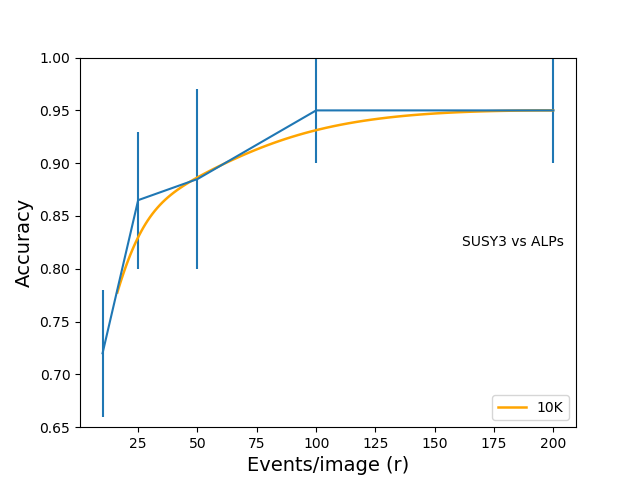
\includegraphics[scale=0.50]{figures/accuracyband2dSUSY3vsAxion10k.png}
\caption{Accuracy (and the corresponding error bands) versus number of events per image with the varying total number of events for SUSY3 versus ALP using fully-connected NNs with two hidden layers.} \label{accuracy2}
\end{figure}


\begin{figure}% [H]
\centering
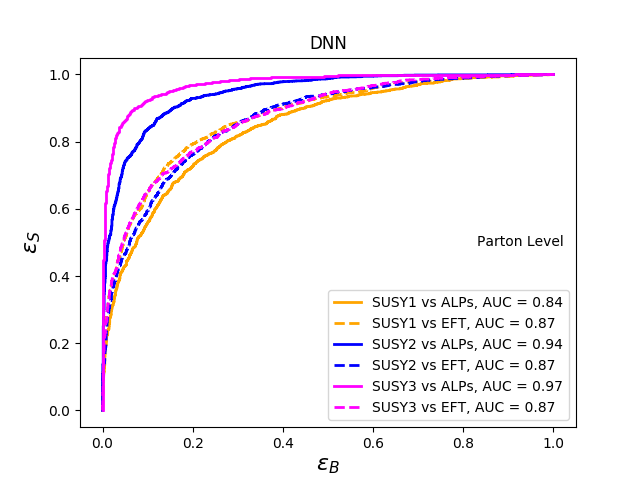
\includegraphics[scale=0.50]{figures/2D_DNN_SUSY_vs_sig_LO_ROC.png}
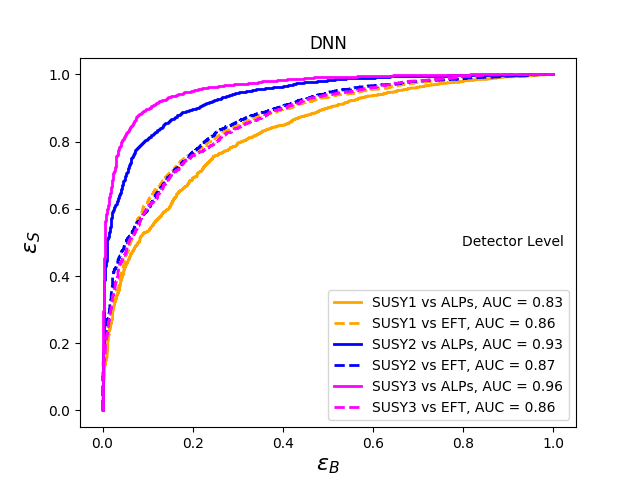
\includegraphics[scale=0.50]{figures/2D_DNN_SUSY_vs_sig_delphes_ROC.png}
\caption{ROC curves (DNN with 2D histograms, $r = 20$) for SUSY WIMP benchmarks versus other signals, for the parton-level (upper) and detector-level (lower) simulations. 200K events are used for each data class sample.}\label{2D_DNN_SUSY_vs_sig_LO_ROC}
\end{figure}


\begin{figure}% [H]
\centering
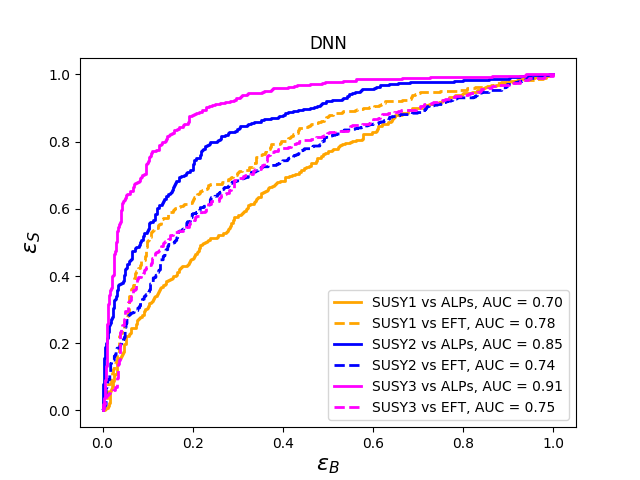
\includegraphics[scale=0.50]{figures/2D_DNN_SUSY_vs_sig_NLO_pt-metphij1_ROC.png}
\caption{ROC curves (DNN with 2D histograms, $r = 20$) for SUSY WIMP versus signal for the dijet NLO detector-level simulation. For these plots, 50K events are used for each process.}\label{2D_DNN_SUSY_vs_sig_NLO_ROC}
\end{figure}




\begin{figure}% [H]
\centering
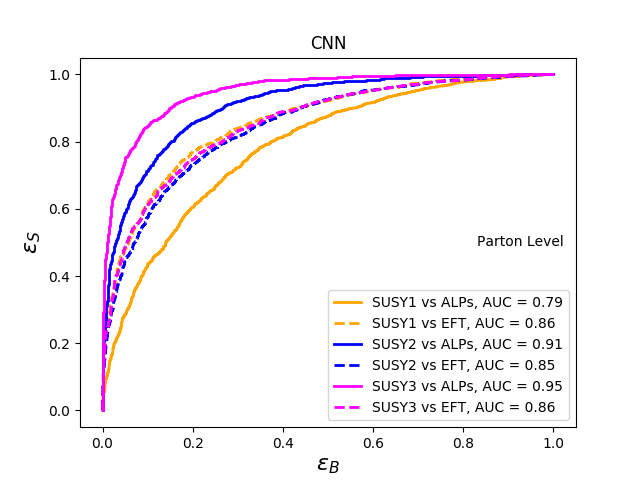
\includegraphics[scale=0.50]{figures/2D_CNN_SUSY_vs_sig_LO_ROC.png}
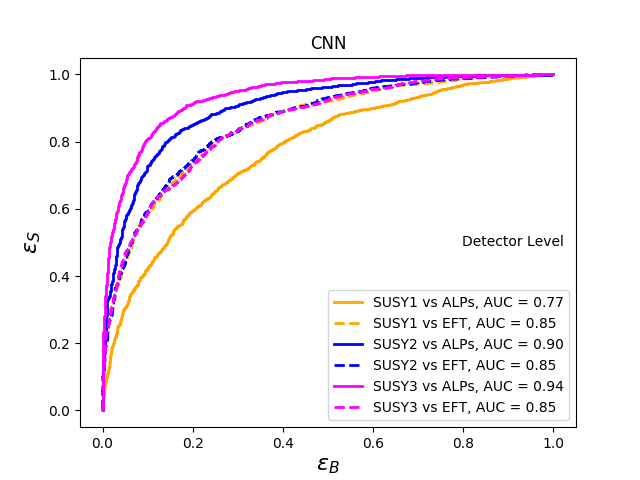
\includegraphics[scale=0.50]{figures/2D_CNN_SUSY_vs_sig_delphes_ROC.png}
\caption{ROC curves (CNN with 2D histograms, $r = 20$) for SUSY benchmarks versus other signals for  parton-level (upper) and detector-level (lower) simulations. For these plots, 200K events are used for each data category.}\label{2D_CNN_SUSY_vs_sig_LO_ROC}
\end{figure}

\begin{figure}% [H]
\centering
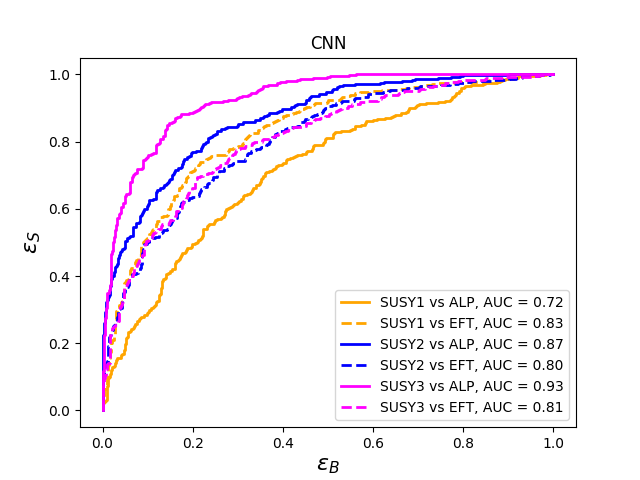
\includegraphics[scale=0.50]{figures/2D_CNN_SUSY_vs_sig_NLO_pt-metphij1_ROC.png}
\caption{ROC curves (CNN with 2D histograms, $r = 20$) for signal versus signal for the dijet NLO detector level simulation. For these plots, 50K events are used for each process.}\label{2D_CNN_SUSY_vs_sig_NLO_ROC}
\end{figure}
%%%%%%%%%%%%%
\section{Conclusions and Outlook}
%%%%%%%%%%%%
In this paper, we used supervised Machine Learning algorithms for the identification of WIMP dark matter in the monojet and missing transverse energy channel. In addition to considering the prospects of detecting WIMP monojet signal over the SM background, we also address the key question of what is the probability that other  signals may mimic WIMP dark matter. We considered LO and NLO parton- detector-level  events for the data samples. We found that for the LO signal there is not a significant degradation in the performance when we perform the realistic detector level analysis.
 
We used different ML approaches to the classification problem: logistic regression, DNNs and CNNs.  We found that for the kinematic variables NN performs better than logistic regression. 

We then created images made of approximations to the probability density of events in a kinematic 2D plane. We then feed the images to a DNN and a CNN. The processing of these images  offers a better classification accuracy  than lists of events with values of kinematic observables.  We found a trade-off between the accuracy and number of events averaged for one histogram. In a more realistic situation, one would expect a small sample of DM events, hence our exploration of low values of  `$r$. 

We also investigated NLO monojet processes and found that the accuracy could increase as compared to the LO monojet, simply because an event with more than one object contains more information. In this case, we performed a PCA analysis to decide the most important combination of features, and then constructed 2D histograms of those.

The techniques proposed could be used for the actual data incorporating the information of the cross-section by choosing specific model benchmarks.  Our study focused instead on features which are independent of these. Nevertheless, one could consider the jet images constructed event-by-event instead of our choice of probability distributions. 

Moreover, this analysis could be extended for other channels in collider dark matter searches, e.g. for the Vector Boson Fusion (VBF) topology where we have two additional forward jets. It would be interesting to compare the performance of proposed methods for the dijet and VBF case. A combined analysis of different channels may offer enhanced sensitivity which will be investigated in the near future. 

Finally, the promising results of this analysis adds a further motivation to explore the possibility of using unsupervised techniques.

\section{acknowledgments}
%\begin{acknowledgments}
C.K.K. wishes to acknowledge support from the Royal Society-SERB Newton International Fellowship (NF171488). 
The work of V.S. by the Science Technology and Facilities Council (STFC) under grant number $\text{ST/P000819/1}$. M.S. wishes to acknowledge the support by the Data Intensive Science Center in the South East Physics Network (DISCnet), an extension of the STFC, under grant number ST/P006760/1. We would also like to thank Alexander Belyaev for his comments on the levels of signal and background.
%\end{acknowledgments}

\appendix
\newcommand{\hbAppendixPrefix}{A}
%
\renewcommand{\thefigure}{\hbAppendixPrefix\arabic{figure}}
\setcounter{figure}{0}

\setcounter{table}{0}
\renewcommand{\thetable}{B\arabic{table}}
%%%%%%%%%%%%%%%%%%%%%%%%%%%%%%%%%%%%%%%%%%%%%%%%%%%
\section{Analysis set-up\label{setup}}
%%%%%%%%%%%%%%%%%%%%%%%%%%%%%%%%%%%%%%%%%%%%%%%%%%%
\subsection{Leading-order(LO) parton-level simulation}
We generate parton-level events for monojet and missing energy signals and centre-of-mass energy $\sqrt{s}=14$ TeV using  MadGraph$\_$aMC$@$NLO v2.6.3.2~\cite{Alwall:2011uj}. 
For SUSY WIMP, we used MSSM-SLHA2 model (all the SUSY spectrum is set to be very heavy except the lightest  neutralino). We use the {\tt Feynrules} model file~\cite{Christensen:2008py,Degrande:2011ua} for the linear ALPs~\cite{linearalps} and  spin-one mediator case (DMsimp$\_$s$\_$spin1~\cite{dmsimp_s_spin1} model) in the EFT framework. 

Using these models, we generate the following processes
\be  p p \rightarrow a j \qquad \mbox{ALPs} \ee
\be  p p \rightarrow \chi \bar \chi j \qquad \mbox{EFT, spin-1 mediator} \ee
\be p p \rightarrow  \tilde \chi^0_1  \tilde \chi^0_1 j \qquad \mbox{SUSY-WIMP}  \ee
For SM monojet background, we consider the following dominant background:
\be  pp \rightarrow Z j (Z \rightarrow \nu\bar\nu). \ee


For all the processes 400K events are generated using a cut of $p_T > 130$ GeV for the jet $p_T$. The following kinematic variables are constructed;
\[p_T^j ({\text{MET}}) ,\eta^j, \phi^j.  \]


\subsection{Leading-order (LO) and Next-to-Leading order (NLO) detector-level simulation}
We generate both monojet and dijet $+$ MET processes. As earlier, hard processes are generated using Madgraph and \textsc{pythia}~\cite{Sjostrand:2007gs} is used for hadronization and showering.
Detector effects are incorporated using \textsc{Delphes}~\cite{deFavereau:2013fsa} with the default ATLAS card. A generation level cut of $p_T^j > 130$ GeV is used for leading jet $p_T$. For the NLO case, while analysing the root file, in addition to the
leading jet $p_T$ cut we also demand $p_T^j > 25$ GeV for the sub-leading jet. 

We have used 200K events for all the cases after root file analysis. To avoid the double-counting from showering, a jet merging scheme (MLM)
with xqcut 20 GeV is applied. For the monojet, we consider the same three kinematic features  as in the parton-level monojet events. For the dijet, we consider 50K events for all the processes and
construct the following kinematic variables :
\begin{itemize}
\item $p_T^{j_1}$: transverse momentum of the leading jet.
\item  $p_T^{j_2}$ transverse momentum of the sub-leading jet. 
\item  $\eta^{j_1}$: pseudo-rapidity of the leading jet.
\item  $\eta^{j_2}$: pseudo-rapidity of the sub-leading jet. 
\item  MET: missing transverse momentum.
\item  $\Delta \phi_{j_1j_2}$: angular separation between the leading and sub-leading jet.
\item  $\Delta \phi_{\text{MET}}^{j_1}$: angular separation between the MET and leading jet.
\item  $\Delta \phi_{\text{MET}}^{j_2}$: angular separation between the MET and sub-leading jet.
\end{itemize}


\begin{figure} [H]
\begin{center}
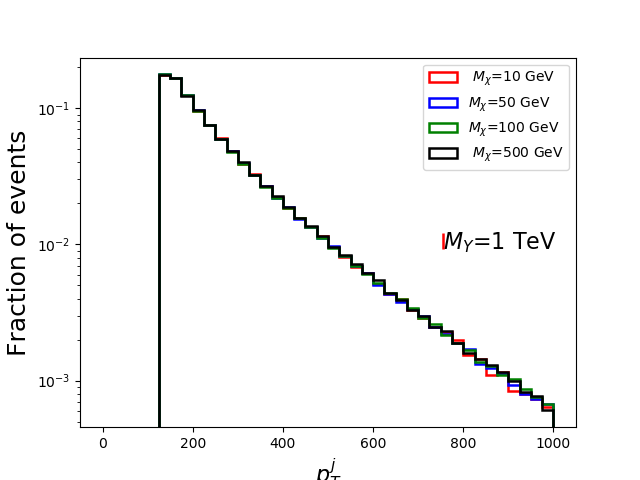
\includegraphics[scale=0.26]{figures/ptjS1med1tev.png}
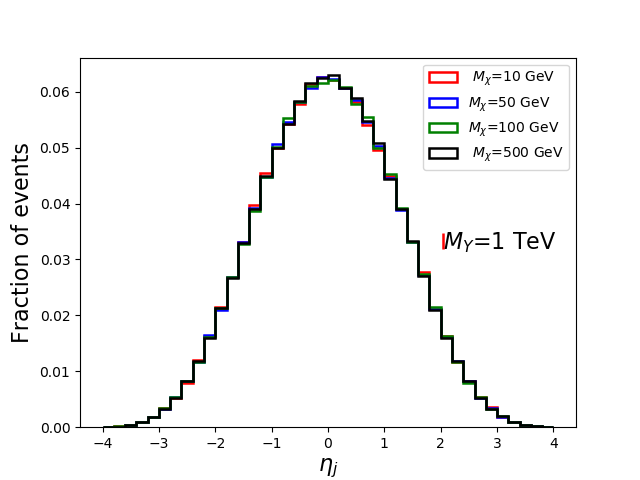
\includegraphics[scale=0.26]{figures/etajS1med1tev.png}
\includegraphics[scale=0.26]{figures/phijS1med1tev.png}
\caption{The $p_T$, $\eta$,  and $\phi$ distributions for the monojet and MET process in case of EFT spin-1 mediator (at parton-level) for fixed mediator mass and  various dark matter masses.\label{spin1med}}
\end{center}
\end{figure}


\section{PCA correlations\label{PCA}}

\begin{figure} [H]
\centering
\includegraphics[scale=0.26]{figures/ALP_PCA.png}
\includegraphics[scale=0.26]{figures/EFT_PCA.png}
\includegraphics[scale=0.26]{figures/SUSY1_PCA.png}
\includegraphics[scale=0.26]{figures/SUSY2_PCA.png}
\caption{The   variance ratio of the new principal component axes (with the number of principal component axes being 8, the same number of original features), highlighting the relative importance of the principal components in terms of capturing variance in the datasets.}\label{PCA_plots2}
\end{figure}





\begin{table}[H]
\scalebox{0.95}{
\begin{tabular}{|c|c|c|c|c|c|c|c|c|}
\hline
\multicolumn{9}{|c|}{ALP PCA correlations} \\
\hline
\toprule
{} &  $p_T^{j_1}$ &  $p_T^{j_2}$ &  $\eta_{j_1}$ &  $\eta_{j_2}$ &  $\Delta \phi_{j_1j_2}$ &   $\text{MET}$ &  $\Delta \phi_{\text{MET}}^{j_1}$ &  $\Delta \phi_{\text{MET}}^{j_2}$ \\ \hline
\midrule
PC-1 &  0.66 &  0.36 &   0.01 &   0.00 &  -0.01 &  0.67 &      0.01 &      0.01 \\ \hline
PC-2 & -0.01 &  0.00 &  -0.02 &  -0.02 &  -0.38 & -0.01 &      0.76 &      0.52 \\ \hline
PC-3 &  0.01 & -0.01 &   0.05 &   0.04 &  -0.76 &  0.00 &      0.06 &     -0.64 \\ \hline
PC-4 &  0.00 &  0.00 &  -0.70 &  -0.71 &  -0.04 &  0.00 &     -0.02 &     -0.06 \\ \hline
PC-5 & -0.29 &  0.93 &   0.05 &  -0.04 &  -0.01 & -0.22 &     -0.01 &     -0.01 \\ \hline
PC-6 &  0.02 & -0.06 &   0.71 &  -0.71 &   0.00 &  0.01 &     -0.00 &      0.00 \\ \hline
PC-7 &  0.70 &  0.05 &   0.00 &  -0.00 &   0.00 & -0.71 &     -0.00 &      0.00 \\ \hline
PC-8 &  0.00 & -0.00 &   0.00 &   0.00 &   0.52 & -0.00 &      0.64 &     -0.56 \\ \hline
\bottomrule
\end{tabular}}
\caption{PCA original feature to principal component correlations for the ALPs (rounded to 2 d.p.).}\label{PCA_table2}
\end{table}

\begin{table}[H]
\scalebox{0.95}{
\begin{tabular}{|c|c|c|c|c|c|c|c|c|}
\hline
\multicolumn{9}{|c|}{EFT PCA correlations} \\
\hline
\toprule
{} &  $p_T^{j_1}$ &  $p_T^{j_2}$ &  $\eta_{j_1}$ &  $\eta_{j_2}$ &  $\Delta \phi_{j_1j_2}$ &   $\text{MET}$ &  $\Delta \phi_{\text{MET}}^{j_1}$ &  $\Delta \phi_{\text{MET}}^{j_2}$ \\ \hline
\midrule
PC-1 &  0.67 &  0.34 &  -0.00 &   0.00 &   0.00 &  0.66 &      0.01 &      0.02 \\ \hline
PC-2 & -0.01 & -0.01 &  -0.00 &   0.01 &  -0.33 & -0.01 &      0.76 &      0.56 \\ \hline
PC-3 &  0.01 & -0.00 &   0.00 &   0.01 &  -0.80 &  0.01 &      0.10 &     -0.59 \\ \hline
PC-4 & -0.00 &  0.01 &   0.71 &   0.71 &   0.01 & -0.00 &     -0.00 &      0.00 \\ \hline
PC-5 & -0.22 &  0.94 &  -0.03 &   0.02 &  -0.01 & -0.27 &      0.00 &     -0.00 \\ \hline
PC-6 &  0.01 & -0.04 &  -0.71 &   0.71 &   0.01 &  0.01 &     -0.01 &      0.00 \\ \hline
PC-7 & -0.71 &  0.04 &   0.00 &  -0.00 &  -0.00 &  0.70 &     -0.00 &     -0.00 \\ \hline
PC-8 & -0.00 &  0.00 &  -0.00 &   0.00 &   0.51 &  0.00 &      0.64 &     -0.57 \\ \hline
\bottomrule
\end{tabular}}
\caption{PCA original features to principal component correlations for the EFT simplified framework (rounded to 2 d.p.).}\label{PCA_table3}
\end{table}


\begin{table}[H]
\scalebox{0.95}{
\begin{tabular}{|c|c|c|c|c|c|c|c|c|}
\hline
\multicolumn{9}{|c|}{SUSY1, $M_{\tilde{\chi}_1^0} = 100$ GeV PCA correlations} \\
\hline
\toprule
{} &  $p_T^{j_1}$ &  $p_T^{j_2}$ &  $\eta_{j_1}$ &  $\eta_{j_2}$ &  $\Delta \phi_{j_1j_2}$ &   $\text{MET}$ &  $\Delta \phi_{\text{MET}}^{j_1}$ &  $\Delta \phi_{\text{MET}}^{j_2}$ \\ \hline
\midrule
PC-1 &  0.67 &  0.35 &   0.01 &   0.00 &  -0.00 &  0.66 &      0.01 &      0.00 \\ \hline
PC-2 &  0.00 &  0.01 &  -0.01 &  -0.01 &   0.37 &  0.00 &     -0.76 &     -0.53 \\ \hline
PC-3 &  0.00 & -0.02 &  -0.01 &  -0.01 &   0.77 &  0.01 &     -0.07 &      0.63 \\ \hline
PC-4 & -0.00 & -0.01 &   0.71 &   0.71 &   0.01 & -0.00 &     -0.01 &     -0.00 \\ \hline
PC-5 & -0.21 &  0.93 &  -0.03 &   0.04 &   0.01 & -0.28 &      0.00 &      0.01 \\ \hline
PC-6 & -0.01 &  0.05 &   0.71 &  -0.71 &   0.00 & -0.02 &     -0.00 &     -0.00 \\ \hline
PC-7 &  0.71 & -0.05 &  -0.00 &  -0.00 &   0.00 & -0.70 &     -0.00 &      0.00 \\ \hline
PC-8 &  0.00 &  0.00 &   0.00 &   0.00 &  -0.52 & -0.00 &     -0.65 &      0.56 \\ \hline
\bottomrule
\end{tabular}}
\caption{PCA original features to principal component correlations for the SUSY1 case (rounded to 2 d.p.).}\label{PCA_table4}
\end{table}


\begin{table}[H]
\scalebox{0.95}{
\begin{tabular}{|c|c|c|c|c|c|c|c|c|}
\hline
\multicolumn{9}{|c|}{SUSY2, $M_{\tilde{\chi}_1^0} = 200$ GeV PCA correlations} \\
\hline
\toprule
{} &  $p_T^{j_1}$ &  $p_T^{j_2}$ &  $\eta_{j_1}$ &  $\eta_{j_2}$ &  $\Delta \phi_{j_1j_2}$ &   $\text{MET}$ &  $\Delta \phi_{\text{MET}}^{j_1}$ &  $\Delta \phi_{\text{MET}}^{j_2}$ \\ \hline
\midrule
PC-1 &  0.67 &  0.32 &   0.00 &  -0.00 &  -0.01 &  0.67 &      0.01 &      0.01 \\ \hline
PC-2 &  0.01 &  0.01 &   0.00 &  -0.01 &   0.34 &  0.01 &     -0.76 &     -0.56 \\ \hline
PC-3 & -0.00 &  0.01 &   0.03 &   0.06 &   0.79 & -0.00 &     -0.09 &      0.60 \\ \hline
PC-4 &  0.00 & -0.01 &   0.71 &   0.70 &  -0.05 &  0.00 &      0.00 &     -0.04 \\ \hline
PC-5 & -0.22 &  0.95 &   0.01 &   0.01 &  -0.01 & -0.24 &      0.00 &     -0.01 \\ \hline
PC-6 &  0.00 &  0.00 &  -0.71 &   0.71 &  -0.01 &  0.00 &     -0.00 &     -0.01 \\ \hline
PC-7 &  0.71 & -0.01 &   0.00 &  -0.00 &   0.00 & -0.71 &     -0.00 &     -0.00 \\ \hline
PC-8 &  0.00 &  0.00 &  -0.00 &   0.00 &   0.51 & -0.00 &      0.65 &     -0.57 \\ \hline
\bottomrule
\end{tabular}}
\caption{PCA original features to principal component correlations for the SUSY2 case (rounded to 2 d.p.).}\label{PCA_table5}
\end{table}




\begin{thebibliography}{99}

%\bibitem{Sirunyan:2018gdw} {\bfseries MISSING REFERENCE!!!}

\bibitem{No:2019gvl}
  J.~M.~No, P.~Tunney and B.~Zaldivar,
  %``Probing Dark Matter freeze-in with long-lived particle signatures: MATHUSLA, HL-LHC and FCC-hh,''
  arXiv:1908.11387 [hep-ph].  
  
  

\bibitem{Radovic:2018dip}
  A.~Radovic {\it et al.},
  %``Machine learning at the energy and intensity frontiers of particle physics,''
  Nature {\bf 560} (2018) no.7716,  41.
%  doi:10.1038/s41586-018-0361-2





\bibitem{Brehmer:2018eca}
  J.~Brehmer, K.~Cranmer, G.~Louppe and J.~Pavez,
  %``A Guide to Constraining Effective Field Theories with Machine Learning,''
  Phys.\ Rev.\ D {\bf 98} (2018) no.5,  052004,
%  doi:10.1103/PhysRevD.98.052004
  [arXiv:1805.00020 [hep-ph]].
  %%CITATION = doi:10.1103/PhysRevD.98.052004;%%
  %20 citations counted in INSPIRE as of 31 May 2019
  
\bibitem{Brehmer:2018kdj}
  J.~Brehmer, K.~Cranmer, G.~Louppe and J.~Pavez,
  %``Constraining Effective Field Theories with Machine Learning,''
  Phys.\ Rev.\ Lett.\  {\bf 121} (2018) no.11,  111801,
%  doi:10.1103/PhysRevLett.121.111801
  [arXiv:1805.00013 [hep-ph]].  



\bibitem{Freitas:2019hbk}
  F.~F.~Freitas, C.~K.~Khosa and V.~Sanz,
  %``Exploring SMEFT in VH with Machine Learning,''
  Phys.\ Rev.\ D {\bf 100} (2019) 035040,
%  doi:10.1103/PhysRevD.100.035040
  [arXiv:1902.05803 [hep-ph]].
%\cite{Freitas:2019hbk}



\bibitem{toptagger}
  G.~Kasieczka, T.~Plehn, M.~Russell and T.~Schell,
  %``Deep-learning Top Taggers or The End of QCD?,''
  JHEP {\bf 1705} (2017) 006,
%  doi:10.1007/JHEP05(2017)006
  [arXiv:1701.08784 [hep-ph]].

\bibitem{manytagger}
  G.~Kasieczka {\it et al.},
  %``The Machine Learning Landscape of Top Taggers,''
  SciPost Phys.\  {\bf 7} (2019) 014,
%  doi:10.21468/SciPostPhys.7.1.014
  [arXiv:1902.09914 [hep-ph]]. 


\bibitem{Piscopo:2019txs}
  M.~L.~Piscopo, M.~Spannowsky and P.~Waite,
  %``Solving differential equations with neural networks: Applications to the calculation of cosmological phase transitions,''
  Phys.\ Rev.\ D {\bf 100} (2019) no.1,  016002,
%  doi:10.1103/PhysRevD.100.016002
  [arXiv:1902.05563 [hep-ph]].


\bibitem{Caron:2016hib}
  S.~Caron, J.~S.~Kim, K.~Rolbiecki, R.~Ruiz de Austri and B.~Stienen,
  %``The BSM-AI project: SUSY-AI–generalizing LHC limits on supersymmetry with machine learning,''
  Eur.\ Phys.\ J.\ C {\bf 77} (2017) no.4,  257,
%  doi:10.1140/epjc/s10052-017-4814-9
  [arXiv:1605.02797 [hep-ph]].   



\bibitem{q-g-tagging} 
  G.~Kasieczka, N.~Kiefer, T.~Plehn and J.~M.~Thompson,
  %``Quark-Gluon Tagging: Machine Learning vs Detector,''
  SciPost Phys.\  {\bf 6} (2019) 069,
%  doi:10.21468/SciPostPhys.6.6.069
  [arXiv:1812.09223 [hep-ph]].  

\bibitem{Brehmer:2019jyt}
  J.~Brehmer, S.~Mishra-Sharma, J.~Hermans, G.~Louppe and K.~Cranmer,
  %``Mining for Dark Matter Substructure: Inferring subhalo population properties from strong lenses with machine learning,''
  arXiv:1909.02005 [astro-ph.CO].
  %%CITATION = ARXIV:1909.02005;%%
  %1 citations counted in INSPIRE as of 17 Sep 2019


\bibitem{Alexander:2019puy}
  S.~Alexander, S.~Gleyzer, E.~McDonough, M.~W.~Toomey and E.~Usai,
  %``Deep Learning the Morphology of Dark Matter Substructure,''
  arXiv:1909.07346 [astro-ph.CO].

\bibitem{cosmoDM}
  C.~Escamilla-Rivera, M.~A.~C.~Quintero and S.~Capozziello,
  %``A deep learning approach to cosmological dark energy models,''
  arXiv:1910.02788 [astro-ph.CO].
  
\bibitem{Simola:2018ntn}
  U.~Simola, B.~Pelssers, D.~Barge, J.~Conrad and J.~Corander,
  %``Machine Learning Accelerated Likelihood-Free Event Reconstruction in Dark Matter Direct Detection,''
  JINST {\bf 14} (2019) no.03,  P03004,
  [arXiv:1810.09930 [astro-ph.IM]].  
  
\bibitem{Mimasu:2014nea}
  K.~Mimasu and V.~Sanz,
  %``ALPs at Colliders,''
  JHEP {\bf 1506} (2015) 173,
%  doi:10.1007/JHEP06(2015)173
  [arXiv:1409.4792 [hep-ph]].
  %%CITATION = doi:10.1007/JHEP06(2015)173;%%

\bibitem{Brivio:2017ije}
  I.~Brivio, M.~B.~Gavela, L.~Merlo, K.~Mimasu, J.~M.~No, R.~del Rey and V.~Sanz,
  %``ALPs Effective Field Theory and Collider Signatures,''
  Eur.\ Phys.\ J.\ C {\bf 77} (2017) no.8,  572,
%  doi:10.1140/epjc/s10052-017-5111-3
  [arXiv:1701.05379 [hep-ph]].
  %%CITATION = doi:10.1140/epjc/s10052-017-5111-3;%%
  %37 citations counted in INSPIRE as of 08 Mar 2019

\bibitem{Barducci:2015ffa}
  D.~Barducci, A.~Belyaev, A.~K.~M.~Bharucha, W.~Porod and V.~Sanz,
  %``Uncovering Natural Supersymmetry via the interplay between the LHC and Direct Dark Matter Detection,''
  JHEP {\bf 1507} (2015) 066,
%  doi:10.1007/JHEP07(2015)066
  [arXiv:1504.02472 [hep-ph]].

\bibitem{Lee:2012ph}
  H.~M.~Lee, M.~Park and V.~Sanz,
  %``Interplay between Fermi gamma-ray lines and collider searches,''
  JHEP {\bf 1303} (2013) 052,
%  doi:10.1007/JHEP03(2013)052
  [arXiv:1212.5647 [hep-ph]].

\bibitem{Gavela:2019cmq} 
  M.~B.~Gavela, J.~M.~No, V.~Sanz and J.~F.~de Trocóniz,
  %``Non-Resonant Searches for Axion-Like Particles at the LHC,''
  arXiv:1905.12953 [hep-ph].
  %%CITATION = ARXIV:1905.12953;%%


\bibitem{2D} 
  F.~Ferreira, S.~Fichet and V.~Sanz,
  %``On new physics searches with multidimensional differential shapes,''
  Phys.\ Lett.\ B {\bf 778}, 35 (2018)
  doi:10.1016/j.physletb.2018.01.008
  [arXiv:1702.05106 [hep-ph]].
  %%CITATION = doi:10.1016/j.physletb.2018.01.008;%%
  %6 citations counted in INSPIRE as of 14 Oct 2019
  
\bibitem{Alwall:2011uj}
  J.~Alwall, M.~Herquet, F.~Maltoni, O.~Mattelaer and T.~Stelzer,
  %``MadGraph 5 : Going Beyond,''
  JHEP {\bf 1106} (2011) 128,
%  doi:10.1007/JHEP06(2011)128
  [arXiv:1106.0522 [hep-ph]].
  %%CITATION = doi:10.1007/JHEP06(2011)128;%%
  
\bibitem{Christensen:2008py}
  N.~D.~Christensen and C.~Duhr,
  %``FeynRules - Feynman rules made easy,''
  Comput.\ Phys.\ Commun.\  {\bf 180} (2009) 1614,
%  doi:10.1016/j.cpc.2009.02.018
  [arXiv:0806.4194 [hep-ph]].

\bibitem{Degrande:2011ua}
  C.~Degrande, C.~Duhr, B.~Fuks, D.~Grellscheid, O.~Mattelaer and T.~Reiter,
  %``UFO - The Universal FeynRules Output,''
  Comput.\ Phys.\ Commun.\  {\bf 183} (2012) 1201,
%  doi:10.1016/j.cpc.2012.01.022
  [arXiv:1108.2040 [hep-ph]].

\bibitem{linearalps} 
http://feynrules.irmp.ucl.ac.be/wiki/ALPsEFT

\bibitem{dmsimp_s_spin1}
http://feynrules.irmp.ucl.ac.be/wiki/DMsimp


  
\bibitem{Sjostrand:2007gs}
  T.~Sjostrand, S.~Mrenna and P.~Z.~Skands,
  %``A Brief Introduction to PYTHIA 8.1,''
  Comput.\ Phys.\ Commun.\  {\bf 178} (2008) 852,
%  doi:10.1016/j.cpc.2008.01.036
  [arXiv:0710.3820 [hep-ph]].
  %%CITATION = doi:10.1016/j.cpc.2008.01.036;%%
  %4619 citations counted in INSPIRE as of 14 Oct 2019  
  
\bibitem{deFavereau:2013fsa}
  J.~de Favereau {\it et al.} [DELPHES 3 Collaboration],
  %``DELPHES 3, A modular framework for fast simulation of a generic collider experiment,''
  JHEP {\bf 1402} (2014) 057,
%  doi:10.1007/JHEP02(2014)057
  [arXiv:1307.6346 [hep-ex]].
  %%CITATION = doi:10.1007/JHEP02(2014)057;%%  
  
\end{thebibliography}

\end{document}
 
